\documentclass[abstract=on,10pt,a4paper,bibliography=totocnumbered]{article}
\usepackage[paper=a4paper,left=35mm,right=35mm,top=25mm,bottom=30mm]{geometry}
\usepackage[doublespacing]{setspace}
\usepackage[english]{babel}
\usepackage[utf8]{inputenc}
\usepackage[round]{natbib}
\usepackage{amsmath}
\usepackage{colortbl}
\usepackage{amsfonts}
\usepackage{amssymb}
\usepackage{gensymb}
\usepackage{graphicx}
\usepackage{tikz}
\usepackage{enumerate}
\usepackage{enumitem}
\usepackage{subcaption}
\usepackage{booktabs}
\usepackage[hidelinks]{hyperref}
\usepackage[nameinlink]{cleveref}
% \usepackage{lineno}
\usepackage{multirow}
\usepackage{arydshln}
\usepackage[flushleft]{threeparttable}
\usepackage[nomarkers, nolists]{endfloat}
\usepackage[colorinlistoftodos]{todonotes}
\usepackage{scalerel}
\usepackage{tikz}
\usetikzlibrary{svg.path}

%------------------------------------------------------------------------------
%	Some Styling
%------------------------------------------------------------------------------
% Creating some TikZ styles
\tikzset{
  nonterminal/.style = {rectangle
    , minimum size = 6mm
    , very thick
    , draw = black!
  }
}

% Changing the style of captions in figures etc.
\captionsetup{labelfont=bf, format=plain, font=small}

% Change how equations are referenced
\renewcommand{\theequation}{Equation \arabic{equation}}%

% To be able to put an ORCID
\definecolor{orcidlogocol}{HTML}{A6CE39}
\tikzset{
  orcidlogo/.pic={
    \fill[orcidlogocol] svg{M256,128c0,70.7-57.3,128-128,128C57.3,256,0,198.7,0,128C0,57.3,57.3,0,128,0C198.7,0,256,57.3,256,128z};
    \fill[white] svg{M86.3,186.2H70.9V79.1h15.4v48.4V186.2z}
                 svg{M108.9,79.1h41.6c39.6,0,57,28.3,57,53.6c0,27.5-21.5,53.6-56.8,53.6h-41.8V79.1z M124.3,172.4h24.5c34.9,0,42.9-26.5,42.9-39.7c0-21.5-13.7-39.7-43.7-39.7h-23.7V172.4z}
                 svg{M88.7,56.8c0,5.5-4.5,10.1-10.1,10.1c-5.6,0-10.1-4.6-10.1-10.1c0-5.6,4.5-10.1,10.1-10.1C84.2,46.7,88.7,51.3,88.7,56.8z};
  }
}
\newcommand\orcid[1]{\href{https://orcid.org/#1}{\mbox{\scalerel*{

\begin{tikzpicture}[yscale=-1,transform shape]
  \pic{orcidlogo};
\end{tikzpicture}
}{|}}}}

%------------------------------------------------------------------------------
%	Titlepage: Header
%------------------------------------------------------------------------------
\title{Flooding of the Okavango Delta influences Connectivity for Dispersing
African Wild Dogs}

% List of Authors
\author{
  David D. Hofmann\textsuperscript{1,2,\S} \orcid{0000-0003-3477-4365} \and
  Dominik M. Behr\textsuperscript{1,2} \orcid{0000-0001-7378-8538} \and
  John W. McNutt\textsuperscript{2} \and
  Arpat Ozgul\textsuperscript{1} \orcid{0000-0001-7477-2642} \and
  Gabriele Cozzi\textsuperscript{1,2} \orcid{0000-0002-1744-1940}
}

% Reduce spacing between authors
\makeatletter
\def\and{%
  \end{tabular}%
  \hskip -0.5em \@plus.17fil\relax
  \begin{tabular}[t]{c}}
\makeatother

% Current Date
% \date{\today}

% And here the masterpiece begins
\begin{document}

% Change page numbering
\pagenumbering{gobble}

% Required to be able to cite
\bibliographystyle{apalike}

% Create Titlepage
\maketitle

%------------------------------------------------------------------------------
%	Titlepage: Additional Info
%------------------------------------------------------------------------------
\begin{flushleft}

\vspace{0.5cm}

\textsuperscript{1} Department of Evolutionary Biology and Environmental
Studies, University of Zurich, Winterthurerstarsse 190, 8057 Zurich,
Switzerland.

\textsuperscript{2} Botswana Predator Conservation Program, Private Bag 13,
Maun, Botswana.

\textsuperscript{\S} Corresponding author: david.hofmann2@uzh.ch

\vspace{4cm}

\textbf{Running Title:} Seasonal Flooding of the Okavango Delta and its
Consequences for African Wild Dog Dispersal and Connectivity

\vspace{0.5cm}

\textbf{Keywords:} movement, connectivity, seasonality, dispersal, conservation,
permeability

\end{flushleft}

%------------------------------------------------------------------------------
%	Abstract
%------------------------------------------------------------------------------
\newpage
\begin{abstract}
Climate change is expected to profoundly impact the life history of wild-living
animal populations. While the impact of climate change on the demographics of
local subpopulations has been studied repeatedly, little is known about the
consequences of environmental change on dispersal and connectivity.

We capitalize on a ``natural experimental setup'', the flood-pulse driven
environmental change across the Okavango Delta in northern Botswana, to
investigate the impact of changing environmental conditions on dispersal
patterns and connectivity of the endangered African wild dog (\textit{Lycaon
pictus}). For this, we simulate dispersal trajectories across the landscape
under two extreme environmental scenarios; one assuming a maximum flood extent,
one assuming a minimum flood extent.

During maximum flood, we observe a reduction in connectivity and an increase in
dispersal durations between distinct habitat patches. Notably, dispersal into
the center of the Okavango delta is reduced by 80\% during maximum flooding. At
minimum flooding, conversely, the delta reveals vital dispersal corridors and
increases chances of successful dispersal into neighboring habitat patches.
Concomittantly, dispersal durations to move between patches is reduced at low
flood levels.

Climate change is expected to critically impact the flood-pulsing cycles of the
Okavango delta and may therefore substantially alter landscape connectivity in
this area. Besides a better understanding of the conservation needs for the
African wild dog, our study also presents a first step towards incorporating
environmental changes due to seasonality or climate change in dispersal and
connectivity analyses. Finally, our analysis demonstrates the usefulness of
individual-based dispersal simulations as a pertinent conservation tool to study
impacts of environmental change while accounting for dispersal movements.

\end{abstract}

%------------------------------------------------------------------------------
%	Main Text
%------------------------------------------------------------------------------
\newpage

\onehalfspacing
\tableofcontents
\doublespacing

% Change page numbering
\newpage
\pagenumbering{arabic}

% Create linenumbers
% \linenumbers

\section{Introduction}
\subsection{Climate Change}
Climate change is expected to profoundly impact ecosystems worldwide, with
far-reaching consequences for species living therein (cite IPCC)
\citep{Ozgul.2010, Radchuk.2019}. However, empirical information on species' responses to climate change remains
scarce, especially for regions most vulnerable to altered conditions
\citep{Paniw.2021}.




\subsection{Dispersal}
The lack of knowledge in terms of species ability to cope with climate change is
further compounded by a lack of information on dispersal under changing
environmental conditions \citep{Travis.2013}. By bringing individuals away from
their natal location, dispersal strongly influences population dynamics
\citep{Clobert.2012}; it enables genetic exchange \citep{Frankham.2002,
Leigh.2012, Baguette.2013}, facilitates the colonization of empty habitats
\citep{Gustafson.1996, Hanski.1999b, MacArthur.2001}, and promotes reinforcement
of weakened and small subpopulations \citep{Brown.1977}. Dispersal also serves
as a means to track suitable habitat \citep{Raia.2012} and may thus serve as a
means to mediate the demographic consequences of environmental change
\citep{Hodgson.2009, Travis.2013}. Dispersal is also inextricably linked to the
concept of landscape connectivity, which is generally understood as the degree
by which the landscape facilitates or impedes movements among habitat patches
\citep{Tylor.1993}.

As previously highlighted by \cite{Travis.2013}, climate may affect dispersal
directly, by altering the propensity of individuals to disperse, or indirectly,
through changes in the biophysical environment. Here, we will focus on the
latter and study dispersal prospects under changing environmental conditions.

In spite of its importance for determining population dynamics and landscape
connectivity, our understanding of dispersal and how dispersal is affected by
changing environmental conditions is limited. This is owed to the difficulty of
obtaining data collected on dispersing animals at the appropriate temporal and
spatial scale \citep{Graves.2014, Vasudev.2015} and our inability to project
dispersal prospects under changing environmental conditions into the future.

The ability of species
to persist under these changing conditions depends on the amplitude and speed of
environmental change and species' responses to such changes (cite someone).

It is, in fact, presumed that humanity has already transgressed the planetary
boundary for climate change, therefore triggering irreversible feedbacks in the
biosphere \citep{Rockstrom.2009}.

Cite IPCC, Planetary boundaries, Tucker (step length). Phenological shifts. Cite
Robynne, Arpat, Megan, Dominik, Rabaiotti etc.

\subsection{Connectivity}
Dispersal is an important, if not the important, driver of landscape
connectivity and therefore of major interest to conservation authorities. It has
also been demonstrated that dispersal may lead to population declines in areas
where anthropogenic mortality is high and dispersal prospects low
\citep{Leigh.2012}.

\subsection{Okavango Delta and African Wild Dogs}
The Okavango delta in Southern Africa poses a unique opportunity to study the
impacts of environmetal change on species dispersal ability and connectivity in
large scale natural experiment setup. According to projections by the IPCC,
Botswana and its surroundings are among the most vulnerable to climate change.
While global temperatures are expected to increase by xx degrees until the end
of the 21st century, For example, \cite{Engelbrecht.2015} predicts an increase
between 4 and 6\degree C for regions in southern Africa. One species that
heavily relies on dispersal for long-term persistence and that inhabits such an
arid ecosystem in Southern Africa is the African wild dog (\textit{Lycaon
pictus}). The African wild dog is a lightly built canid lives in cohesive packs
comprising up to 20 individuals. Wild dogs are social breeders and the majority
of reproduction is monopolized by the dominant alpha couple who are supported by
subordinates in taking care of their pups. The species exhibits strong
inbreeding avoidance, hence juvenile individuals born into the pack disperse in
same-sex sibling coalitions after reaching sexual maturity \citep{McNutt.1996,
Behr.2020}. Notably, the African wild dog is the sole extant representative of
its genus and thus considered as high-priority species for conservation efforts
\citep{Leigh.2012}. However, fragmentation and destruction of their historic
habitat may have decreased dispersal success for this species and thus
jeopardizes connectivity \citep{Leigh.2012}. Since the impacts of climate change
are not uniformly distributed across the planet, but particularly pronounced at
high latitudes and arid ecosystems, the species may be seen as most vulnerable
to such ecosystem shifts.

\subsection{Our Study}
Here, we capitalize on a previously parametrized dispersal model and use
dispersal simulations to investigate connectivity patterns for African wild dogs
under two extreme scenarios; one assuming maximum flooding of the Okavango delta
and one assuming minimum flooding of the Okavango delta. Given that water poses
a barrier to dispersing individuals, we anticipate that dispersal prospects and
connectivity during maximum flood are low. During minimum flood, in contrast, we
expect to reveal the presence of several dispersal corridors that may be used to
freely and quickly move between remaining habitat patches.

\section{Materials and Methods}
We conducted all analyses using the programming language \textsf{R}. Any spatial
data manipulation was completed using the \textsf{terra} and \textsf{spatstat}
packages. Several helper functions for the simulation algorithm were written in
\textsf{C++} and imported to R using the \textsf{Rcpp} package. Figures were
generated using \textsf{ggplot2}, \textsf{igraph}, and \textsf{ggnetwork}. All
R-scripts used to conduct our analyses are provided through an online
repository.

\subsection{Study Area}
The study area for this analysis was focused on the Okavango delta (OD) and its
surroundings in Southern Africa, comprising parts of Angola, Namibia, Botswana,
Zimbabwe, and Zambia (\Cref{StudyArea}). The OD is the world's largest inland
delta and the main driver of seasonal environmental change in the region. While
our primary focus lied on the immediate surroundings of the Okavango Delta, we
considered a large rectangular extent stretching from 20\degree 30' E to
26\degree E. (totaling to an area of 300'000 km\textsuperscript{2}) to
accommodate for the long distance dispersal events commonly observed in African
wild dogs (e.g. \citealp{Davies-Mostert.2012, Masenga.2016, Cozzi.2020}). The
flood-pulsing rhythm of the OD is mainly dictated by precipitation in the
catchment areas of the Angolian highlands, where rainwater is collected and
channeled into the OD through the Okavango River. Although precipitation in
Angola peaks between December and March, water only slowly descends through the
Okavango river and its distributaries, reaching the distal ends of the delta in
July or August, where the water percolates at the Thamalakane and Kunyere
Faults. At minimum extent, the flood covers an area of 3'600
km\textsuperscript{2}, during maximum flood more than 9'000
km\textsuperscript{2}. Vegetation in the study area is dominated by mopane
forest, mixed acacia woodland, and grassland. Human influence is low and mainly
concentrated around small villages at the western periphery of the delta as well
as the city of Maun at the south-eastern tip of the OD. Large portions of land
are dedicated national parks, game reserves or forest reserves. The study area
is also part of the world's largest transboundary conservation initiative, the
Kavango-Zambezi Transfrontier Conservation Area, which aims to restore
connectivity between protected areas in Southern Africa.

\begin{figure}
  \begin{center}
  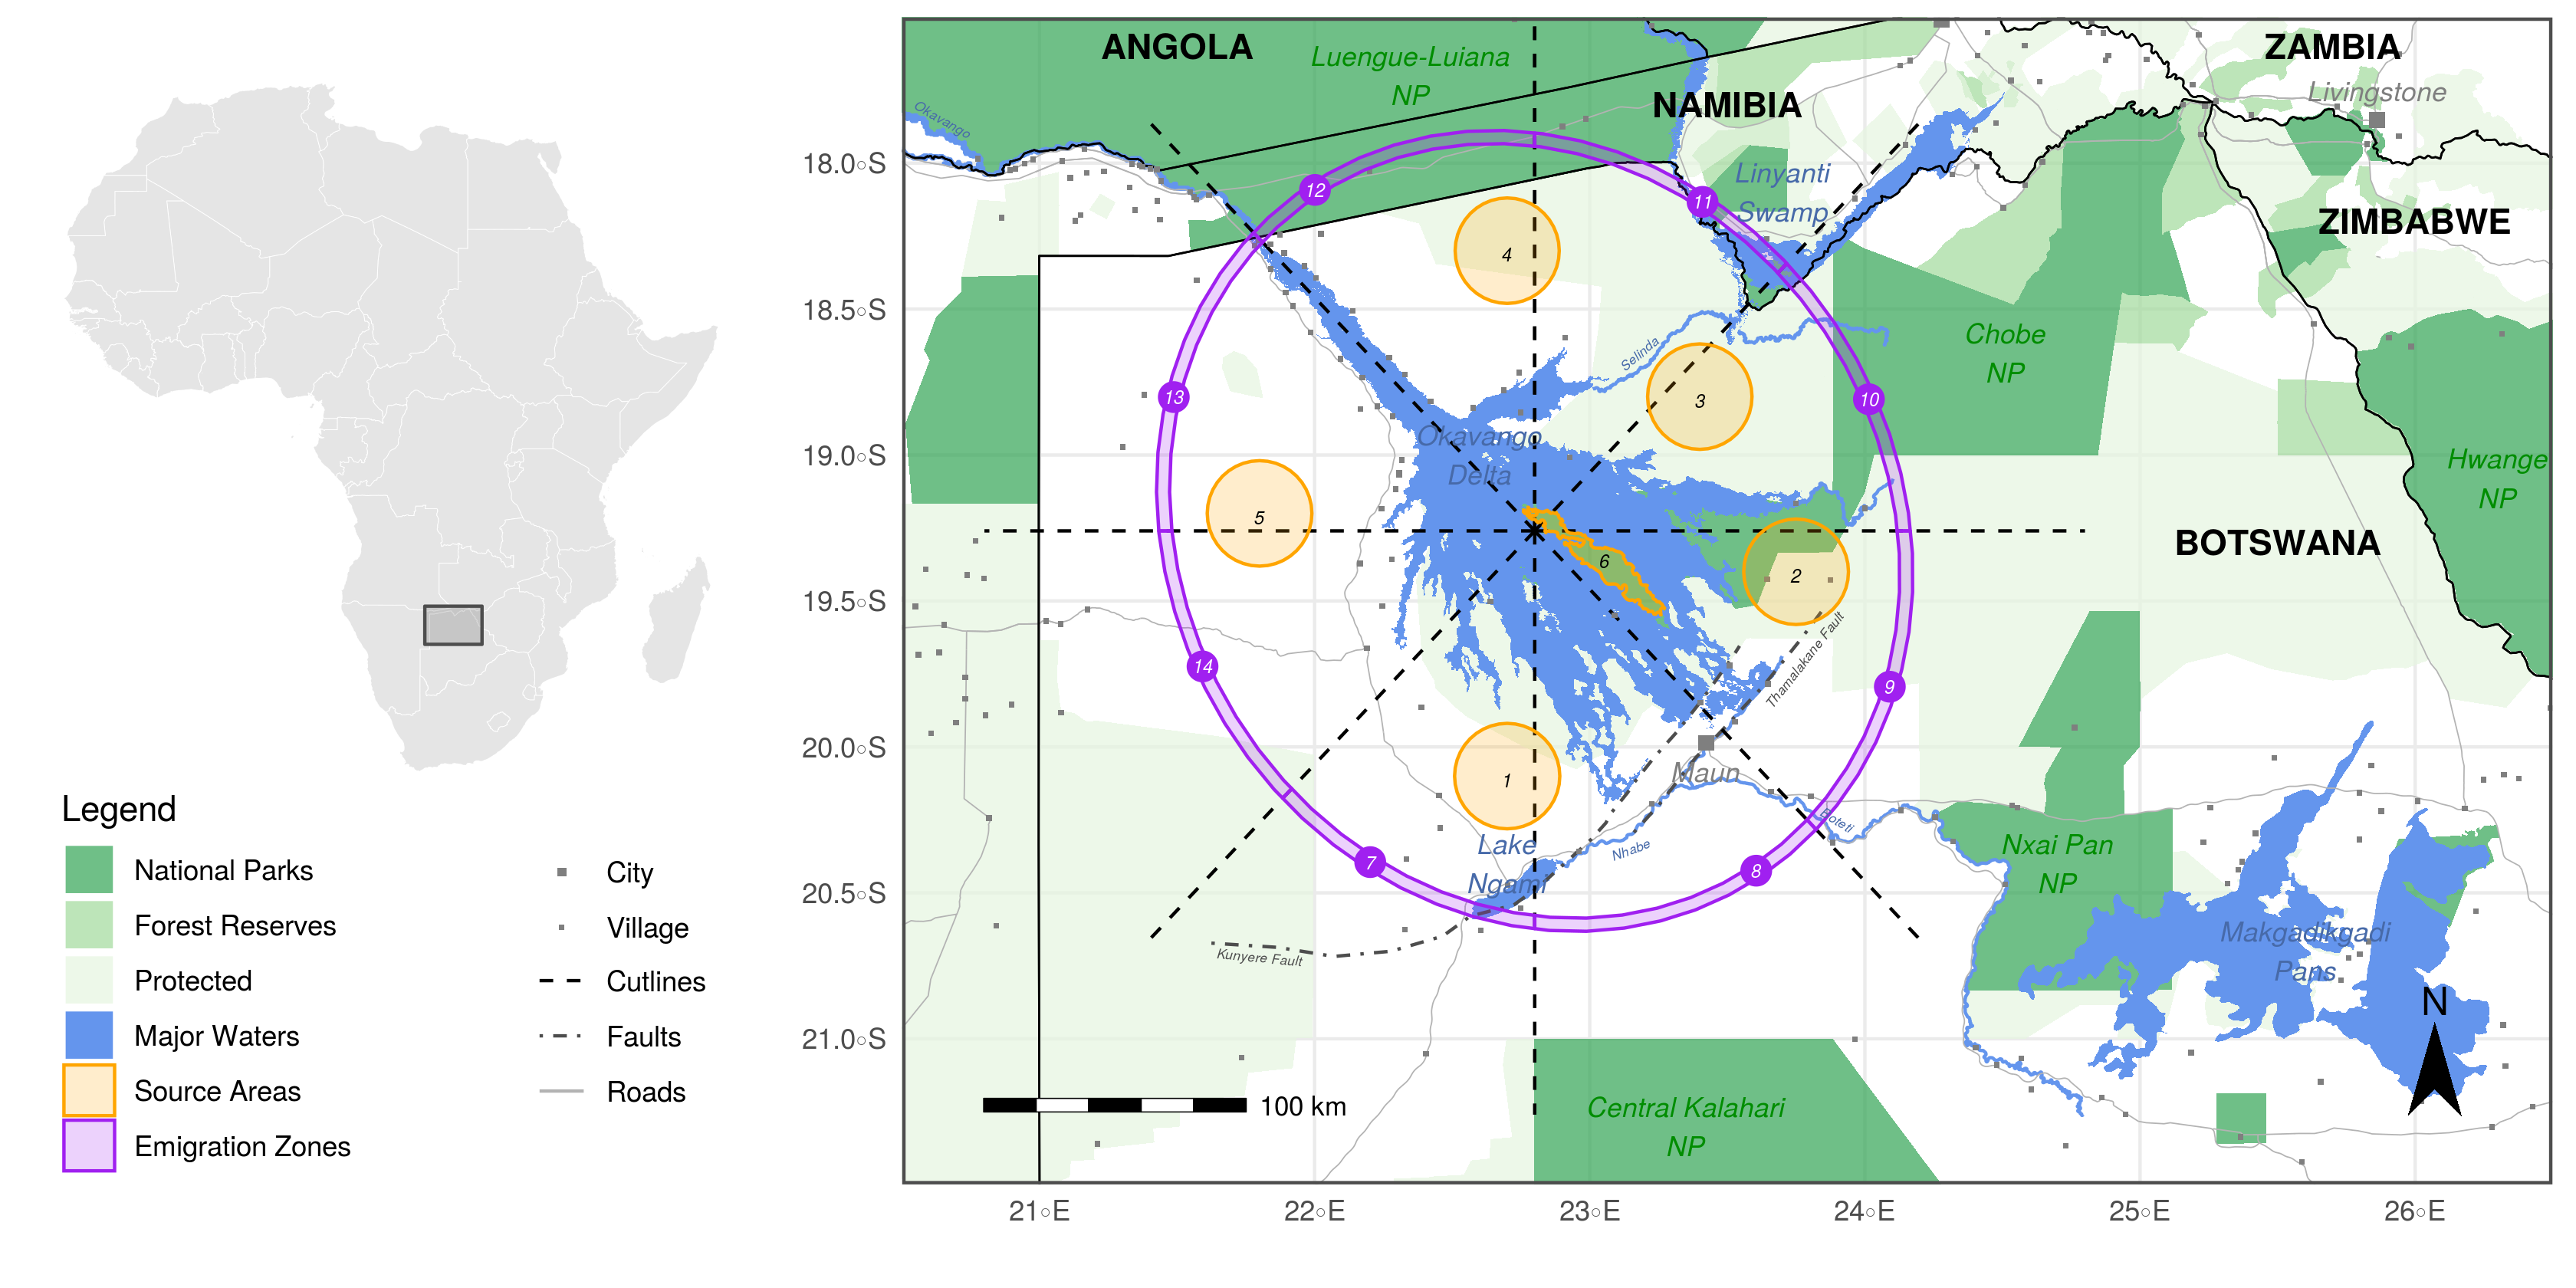
\includegraphics[width = \textwidth]{99_StudyArea.png}
  \caption{Study area across which we simulated dispersal. Simulated dispersers
  were released at random locations within the orange source areas distributed
  across the delta. Emigration zones (purple) served as checkpoints and enabled
  us to identify if and where simulated dispersers left the close surroundings
  of the Okavango delta. These zones were generated using a set of cutlines
  originating from the center of the delta and roughly cutting an elliptical
  buffer zone into sections of equal size.}
  \label{StudyArea}
  \end{center}
\end{figure}

\subsection{Spatial Habitat Layers}
We represented the physical landscape through which dispersers could move by a
set of spatially referenced habitat layers, each resolved at 250m x 250m. The
set of layers included water-cover, distance-to-water, tree-cover,
shrub/grassland-cover, and a human influence layer depicting anthropogenic
influences through villages, roads, and agriculture. A detailed description of
the different habitat layers is provided in \Cref{Hofmann.2021}. Importantly,
the water-cover and derived distance-to water layers were generated using MODIS
Terra MCD43A4 satellite imagery that was classified using a ``floodmapping''
algorithm developed by \citep{Wolski.2017} and available through the R-package
\textsf{floodmapr}. The algorithm allowed us to generate almost weekly updated
``floodmaps'', thus providing detailed information about the flood-extent at any
given point in time. In total, we generated 700 floodmaps between the years 2000
and 2019. Based on these maps, we generated a minimal and maximum flood
scenario. To create the minimum flood scenario, we averaged the 50 floodmaps
with smallest flood extent and generated a binary image using areas that were
inundated in at least 50\% of the maps. Similarly, we created an average image
for high flood using the 50 most flooded maps. The final maps are depicted in
\Cref{FloodExtent}.

\begin{figure}
  \begin{center}
  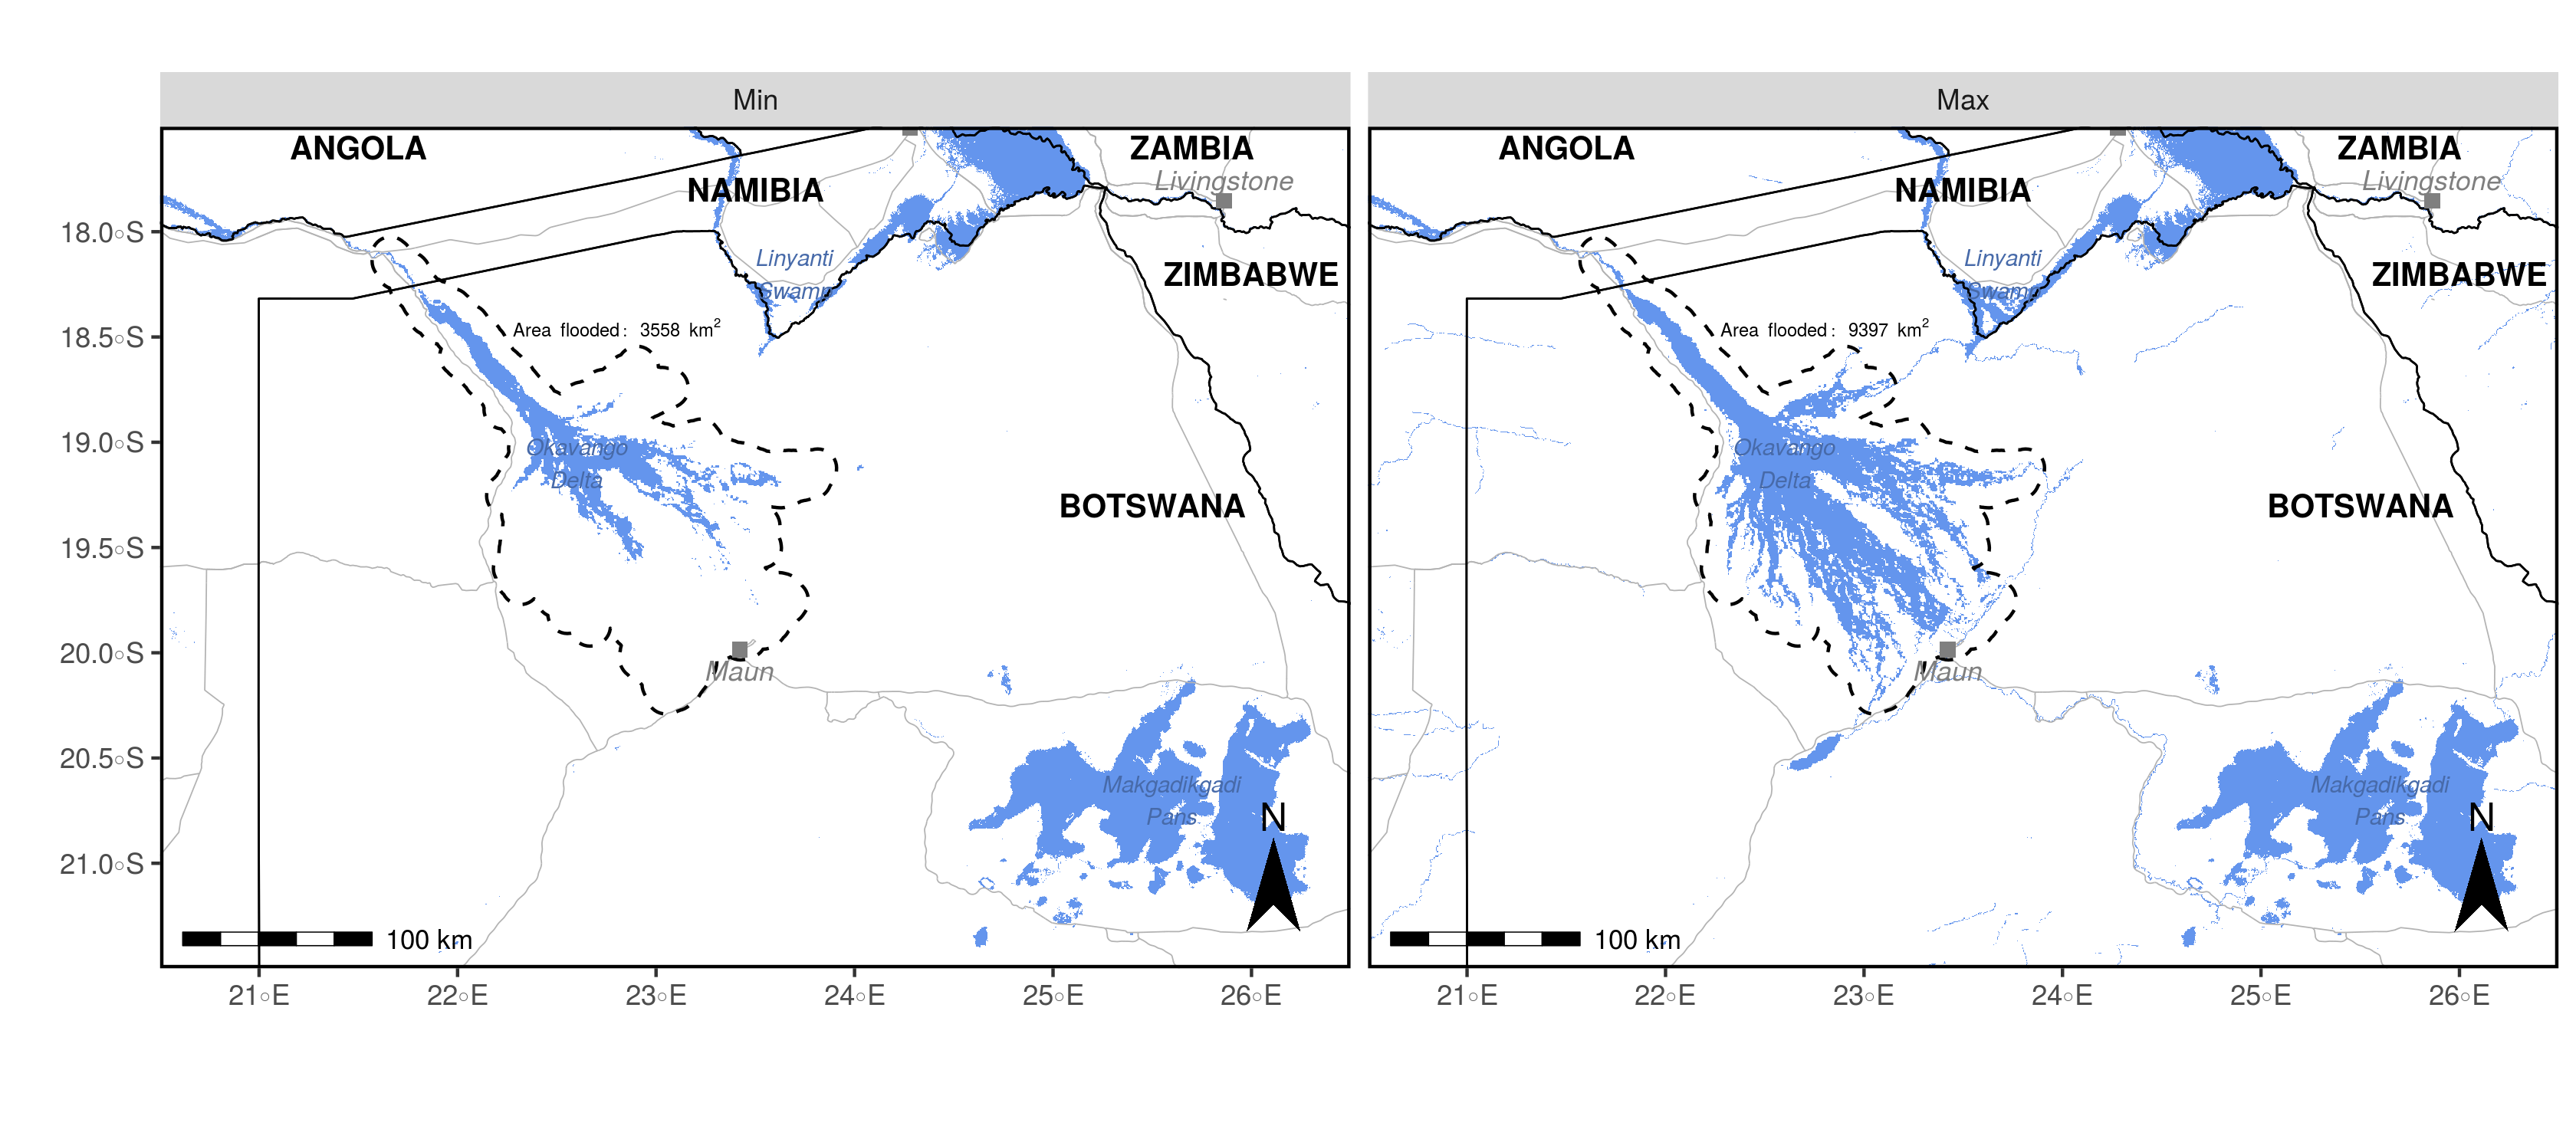
\includegraphics[width = \textwidth]{99_FloodExtent.png}
  \caption{Flood extent in the two scenarios considered. In the left panel, the
  flood is at an extremely low level, stretching across 3'558
  km\textsuperscript{2}, whereas in the right panel the flood is at an extremely
  high level and covers 9'397 km\textsuperscript{2}. The two maps were generated
  using 700 remote sensed MODIS MCD43A4 satellite images spanning the years 2000
  to 2019.}
  \label{FloodExtent}
  \end{center}
\end{figure}

\subsection{Dispersal Model}
Our dispersal model was based on a previously parametrized and validated
integrated step-selection function (iSSF, \citealp{Avgar.2016}) fitted to GPS
data of dispersing AWDs \citep{Hofmann.2021}. In step selection functions (SSFs,
\citealp{Fortin.2005}), observed GPS locations are converted into steps (the
straight-line traveled between two GPS recordings \citep{Turchin.1998a}) and
compared to a set of \textit{random} steps in a (mixed effects) conditional
logistic regression framework \citep{Fortin.2005, Thurfjell.2014, Muff.2020,
Fieberg.2021}. The model presented in \citep{Hofmann.2021} used dispersal data
of 16 dispersing African wild dogs from a free-ranging wild dog population in
northern Botswana. GPS data during dispersal was collected at 4-hourly intervals
and translated into steps of similar duration. Observed steps were then paired
step with 24 random steps that were generated using a uniform distribution for
turning angles (\(-\pi, +\pi\)) and step lengths from a gamma distribution
fitted to observed steps (scale \(\theta\) = 6'308 and shape \(k\) = 0.37). It
was then assumed that animals assigned to each observed and random step a
selection score of the form \citep{Fortin.2005}:

\begin{equation}
\label{EQ1}
  w(x) = exp(\beta_1 x_1 + \beta_2 x_2 + ... + \beta_n x_n)
\end{equation}

Where (\(x_1, x_2, ..., x_n\)) represent the covariate values along each of the
steps and the (\(\beta_1, \beta_2, ..., \beta_n\)) are the animal's relative
selection strengths \citealp{Avgar.2017} towards these covariates. The benefit
of \textit{integrated} SSFs over regular SSFs is that they provide a means to
render two complementary ``kernels''. A movement kernel that describes general
movement behavior of dispersing AWDs and a habitat kernel that describes
preferences of AWDs with regards to environmental conditions
\citep{Fieberg.2021}. iSSFs also allow interactions among the two kernels and
are thus suitable to render that movement behavior may change depending on
habitat conditions. A brief summary of the fitted dispersal model is provided in
Appendix xx.

\subsection{Source Areas and Emigration Zones}
We simulated dispersing AWDs originating from six distinct source areas located
in the vicinity of the Okavango delta (\Cref{StudyArea}). For areas one to six
we selected locations at the delta's periphery that remained dry in both
scenarios. At those locations, we generated circular buffers with a radius of 20
km. For source area six, we isolated a polygon covering Chief's Island, a
peninsula located at the OD's center. Besides source areas, we also generated
``zones of emigration'' that we used as checkpoints to determine if and where
simulated individuals left the delta's vicinity (\Cref{StudyArea}). We generated
emigration zones by first overlaying the OD with an elliptic buffer zone that we
dissected using a set of cutlines that originated from the ODs center and spread
according to cardinal points (\Cref{StudyArea}).

\subsection{Dispersal Simulation}
For each source area we simulated 1'000 individuals, once assuming a minimum
flood, once assuming a maximum flood. This resulted in the simulation of 6'000
individuals for each environmental scenario, hence 12'000 individuals in total.
The simulation algorithm was based on the algorithm described in
\Cref{Hofmann.2022} and works as follows. A random location within the source
area is chosen as a starting point. Originating from the starting point, a set
of 25 random steps is generated by sampling step lengths from a gamma
distribution fitted to observed steps (what is a step?) (shape = , scale = ) and
turning angles from a uniform distibution ($-\pi, +\pi$). Along each random step
the underlying spatial covariates are extracted and relevant movement metrics
are computed (i.e. log(sl), cos(ta), ta). The parametrized dispersal model is
used to predict the probability of each step for being chosen given the steps
covariate values. One of the steps is sampled based on assigned probabilities
and the location of the animal is updated. The procedure is then repated until
the desired number of steps is realized. Here, we simulated each individual for
2'000 steps, which correspons to the longest dispersal duration recorded in our
data. The original model was trained using 4-hourly steps, thus a simulated step
also resembled the movement conducted within four hours. Trajectories resulting
from such a simulation can be understood as correlated random walks that take
into account both habitat and movement preferences of dispersing individuals.

% We used a previously parametrized dispersal model to simulate dispersal
% trajectories of African wild dogs across the study area. To simulate dispersing
% wild dogs, we employed the simulation framework presented in
% \cite{Hofmann.2022}. In this framework, a movement model that renders habitat
% and movement preferences of dispersing individuals is parametrized using
% step-selection functions. Once parametrized, the model can be employed to
% simulate virtual dispersers moving across the landscape.
%
% We released virtual dispersers at random locations within the four distinct
% source areas depicted in \Cref{StudyArea}. From each source area we simulated xx
% individuals moving across the landscape at minimum flood and another xx
% individuals at maximum flood. For comparison, we also ran the simulations for a
% medium flood extent, yet the results for this will be presented in the appendix.

\subsection{Dispersal Prospects and Connectivity}
Based on simulated dispersal trajectories in the two scenarios we quantified
dispersal sucess and connectivity using three complementary connectivity metrics
as outlined in \cite{Hofmann.2022}. First, we generated heatmaps depicting the
frequency at which different areas in the landscape were visited by simulated
dispersers. Such heatmaps serve to detect dispersal hotspots and areas of
intense use. However, they are less suitable for detecting pinchpoints and
bottlenecks that are critical in linking distinct patches. Hence, we also
computed spatially explicit betweenness scores which are useful to highlight
exactly such pinchpoints \citep{Bastille-Rousseau.2018, Bastille-Rousseau.2021}.
To compute betweenness, we overlayed the study area with a regular grid with 2.5
km x 2.5 km grid cells and determined how often simulated individuals
transitioned from one grid-cell to another. Note that in case the same
individual repeatedly realized the same cell-transition (e.g. repeatedly moved
between A-B-A-B...), we only counted a single transition to avoid emphasis on
regions where individuals moved in circles. With on the so generated
transitions, we generated a network using the centers of all grid-cells as nodes
and cell-transitions as weighted connections between the nodes. Based on this
network we computed weighted betweenness scores using the R-package
\textsf{igraph}. As a final connectivity metric and metric of dispersal success,
we calculated the number of successful dispersal events between the different
source areas as well as towards the emigration zones. We coin this type of
connectivity ``inter-patch connectivity'' as it relates to the movement between
distinct patches. Dispersal between two areas was said to be successful whenever
a trajectory leaving one area intersected with the target area. To gauge the
dispersal duration needed to move between patches (be consistent with
``patches'', ``source-areas'' etc.), we also recorded the minimum number of
steps that individuals moved before arriving at the respective patch.

\section{Results}
\subsection{Heatmaps}
Heatmaps produced from simulated dispersal trajectories reveal that the OD acts
as a major dispersal barrier during periods of high flood, but reveals viable
dispersal corridors during periods of low flood (\Cref{Heatmaps}). During
minimum flood, the area north-west of Maun appears to serve as vital dispersal
habitat. The same area is entirely avoided during maximum flood. Besides
striking differences in connectivity for the close vicinity of the delta, the
remainder of the study area shows only marginal differences in connectivity
between the two scenarios. For instance, in both scenarios the area south of the
Linyanti swamp appears as frequently visited dispersal habitat. Additional
heatmaps highlighting differences in connectivity for each source area
separately are provided in Appendix SX.

\begin{figure}
  \begin{center}
  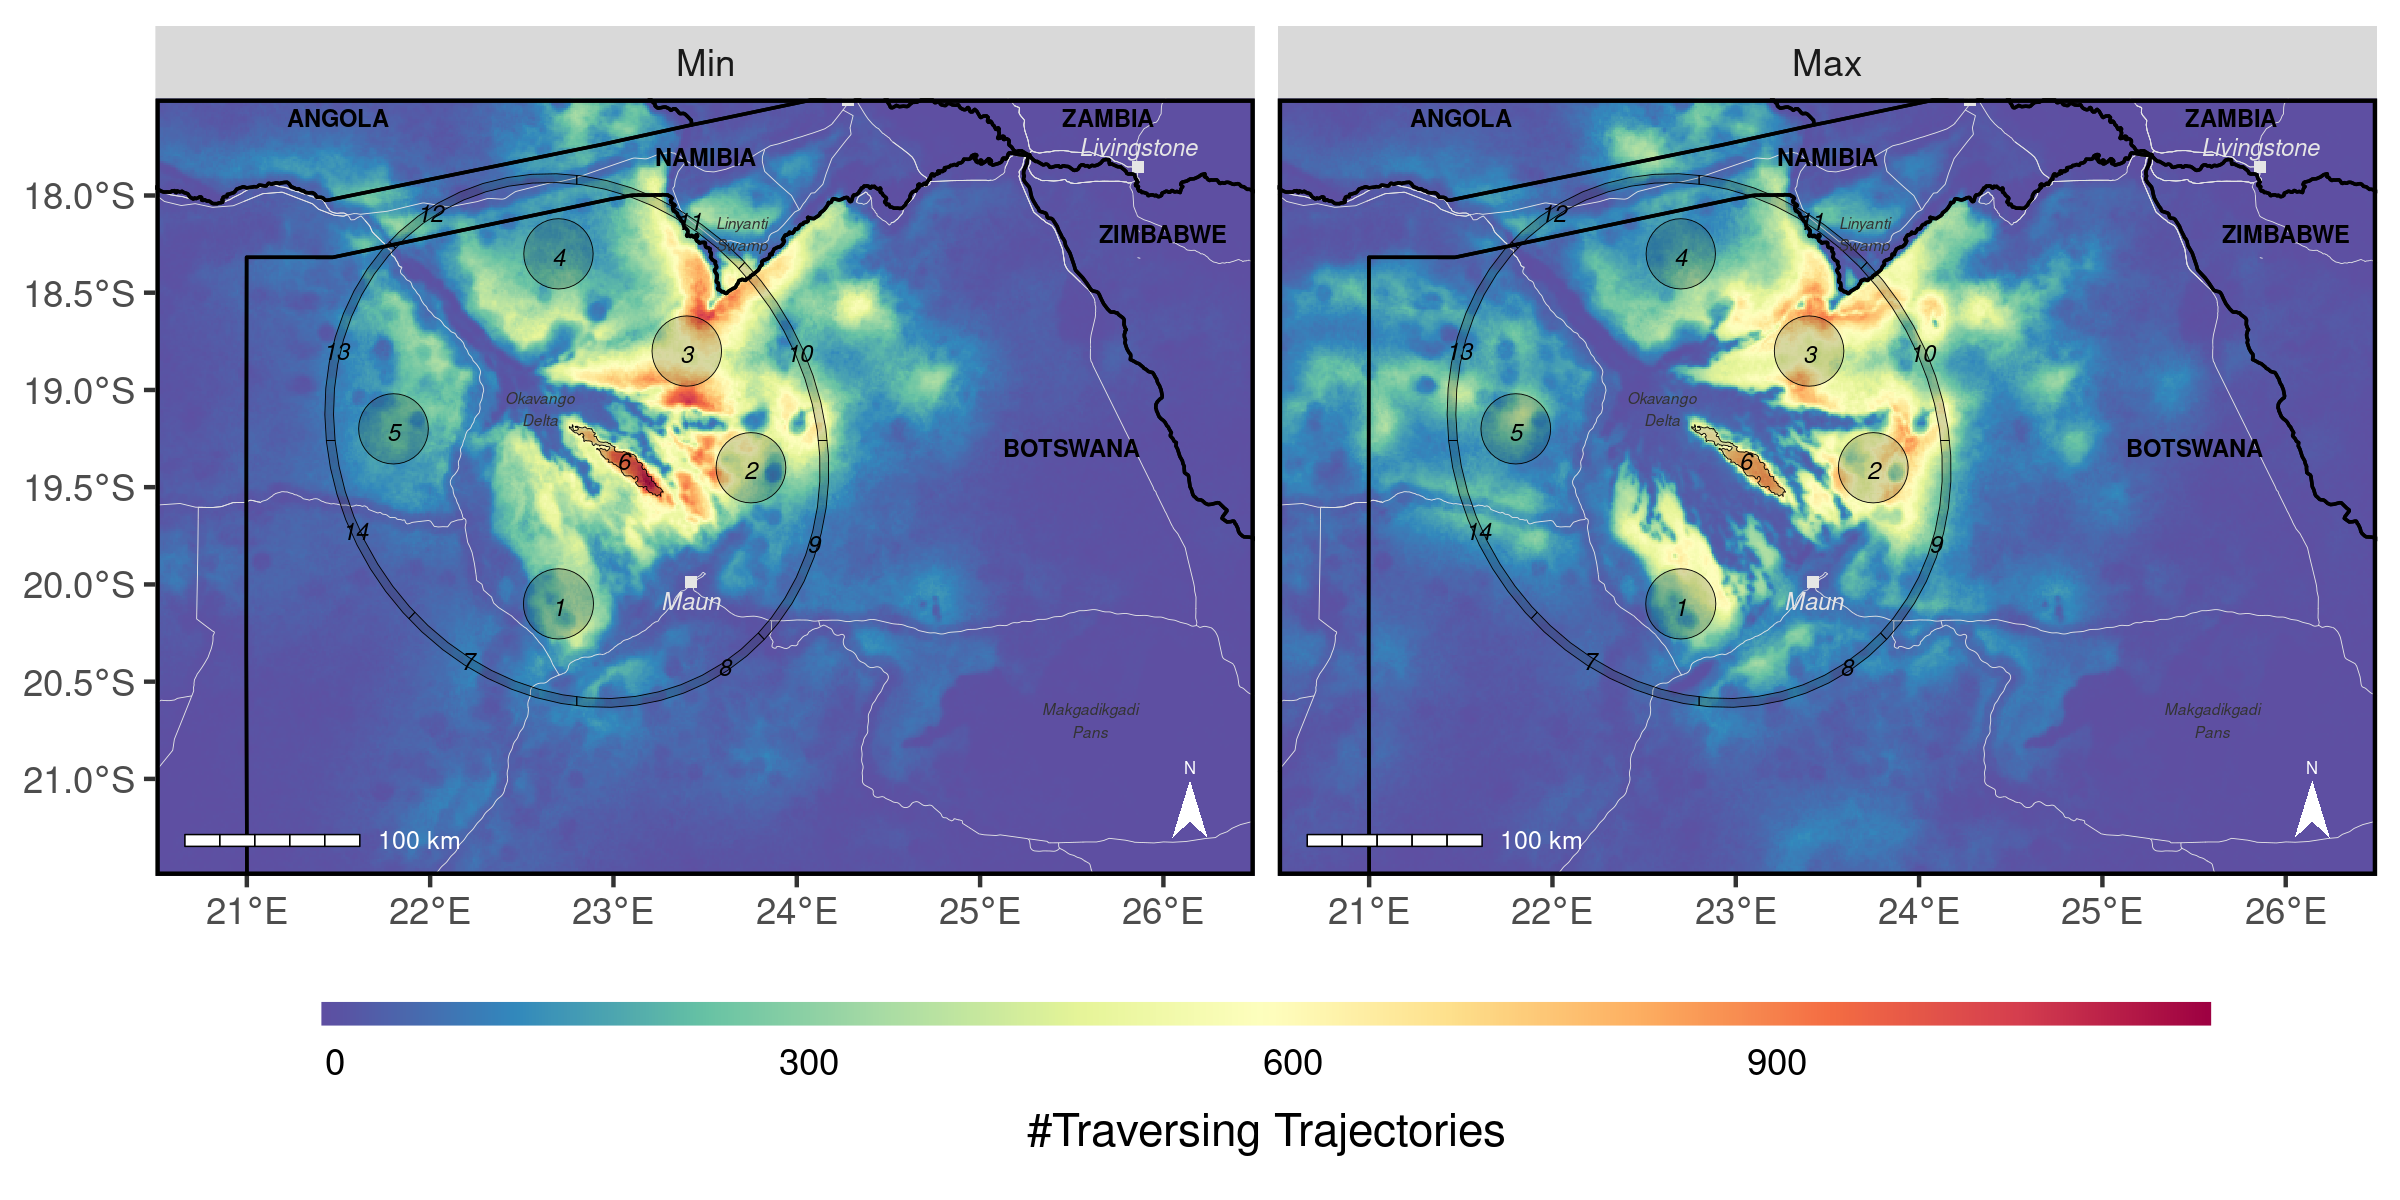
\includegraphics[width = \textwidth]{99_Heatmaps.png}
  \caption{Heatmaps depicting the number of simulated dispersal trajectories
  traversing each grid-cell in the study area. The left panel shows results for
  the minimum flood scenario, whereas the right panel shows results for the
  maximum flood scenario. Source areas (numbered 1-6) from which dispresers were
  released, and emigration zones (numbered 7-14) are shaded in dark gray.}
  \label{Heatmaps}
  \end{center}
\end{figure}

\subsection{Betweenness}
The betweenness maps reveal a similar pattern in that connectivity through the
OD is only pronounced during periods of low floods and vanishes entirely during
maximum flood (\Cref{Betweenness}). A set of four dispersal corridors meets on
the central peninsula (source area 5, \Cref{Betweenness}) at minimum flood but
the same corridors are absent when the flood reaches a maximum extent. Instead,
a narrow corridor runs north west of Maun, connecting source areas one and two.
Again, the remainder of the study area is only marginally affected by flooding
patterns. Additional betweenness maps highlighting differences in connectivity
for each source area separately are provided in Appendix SX.

\begin{figure}
  \begin{center}
  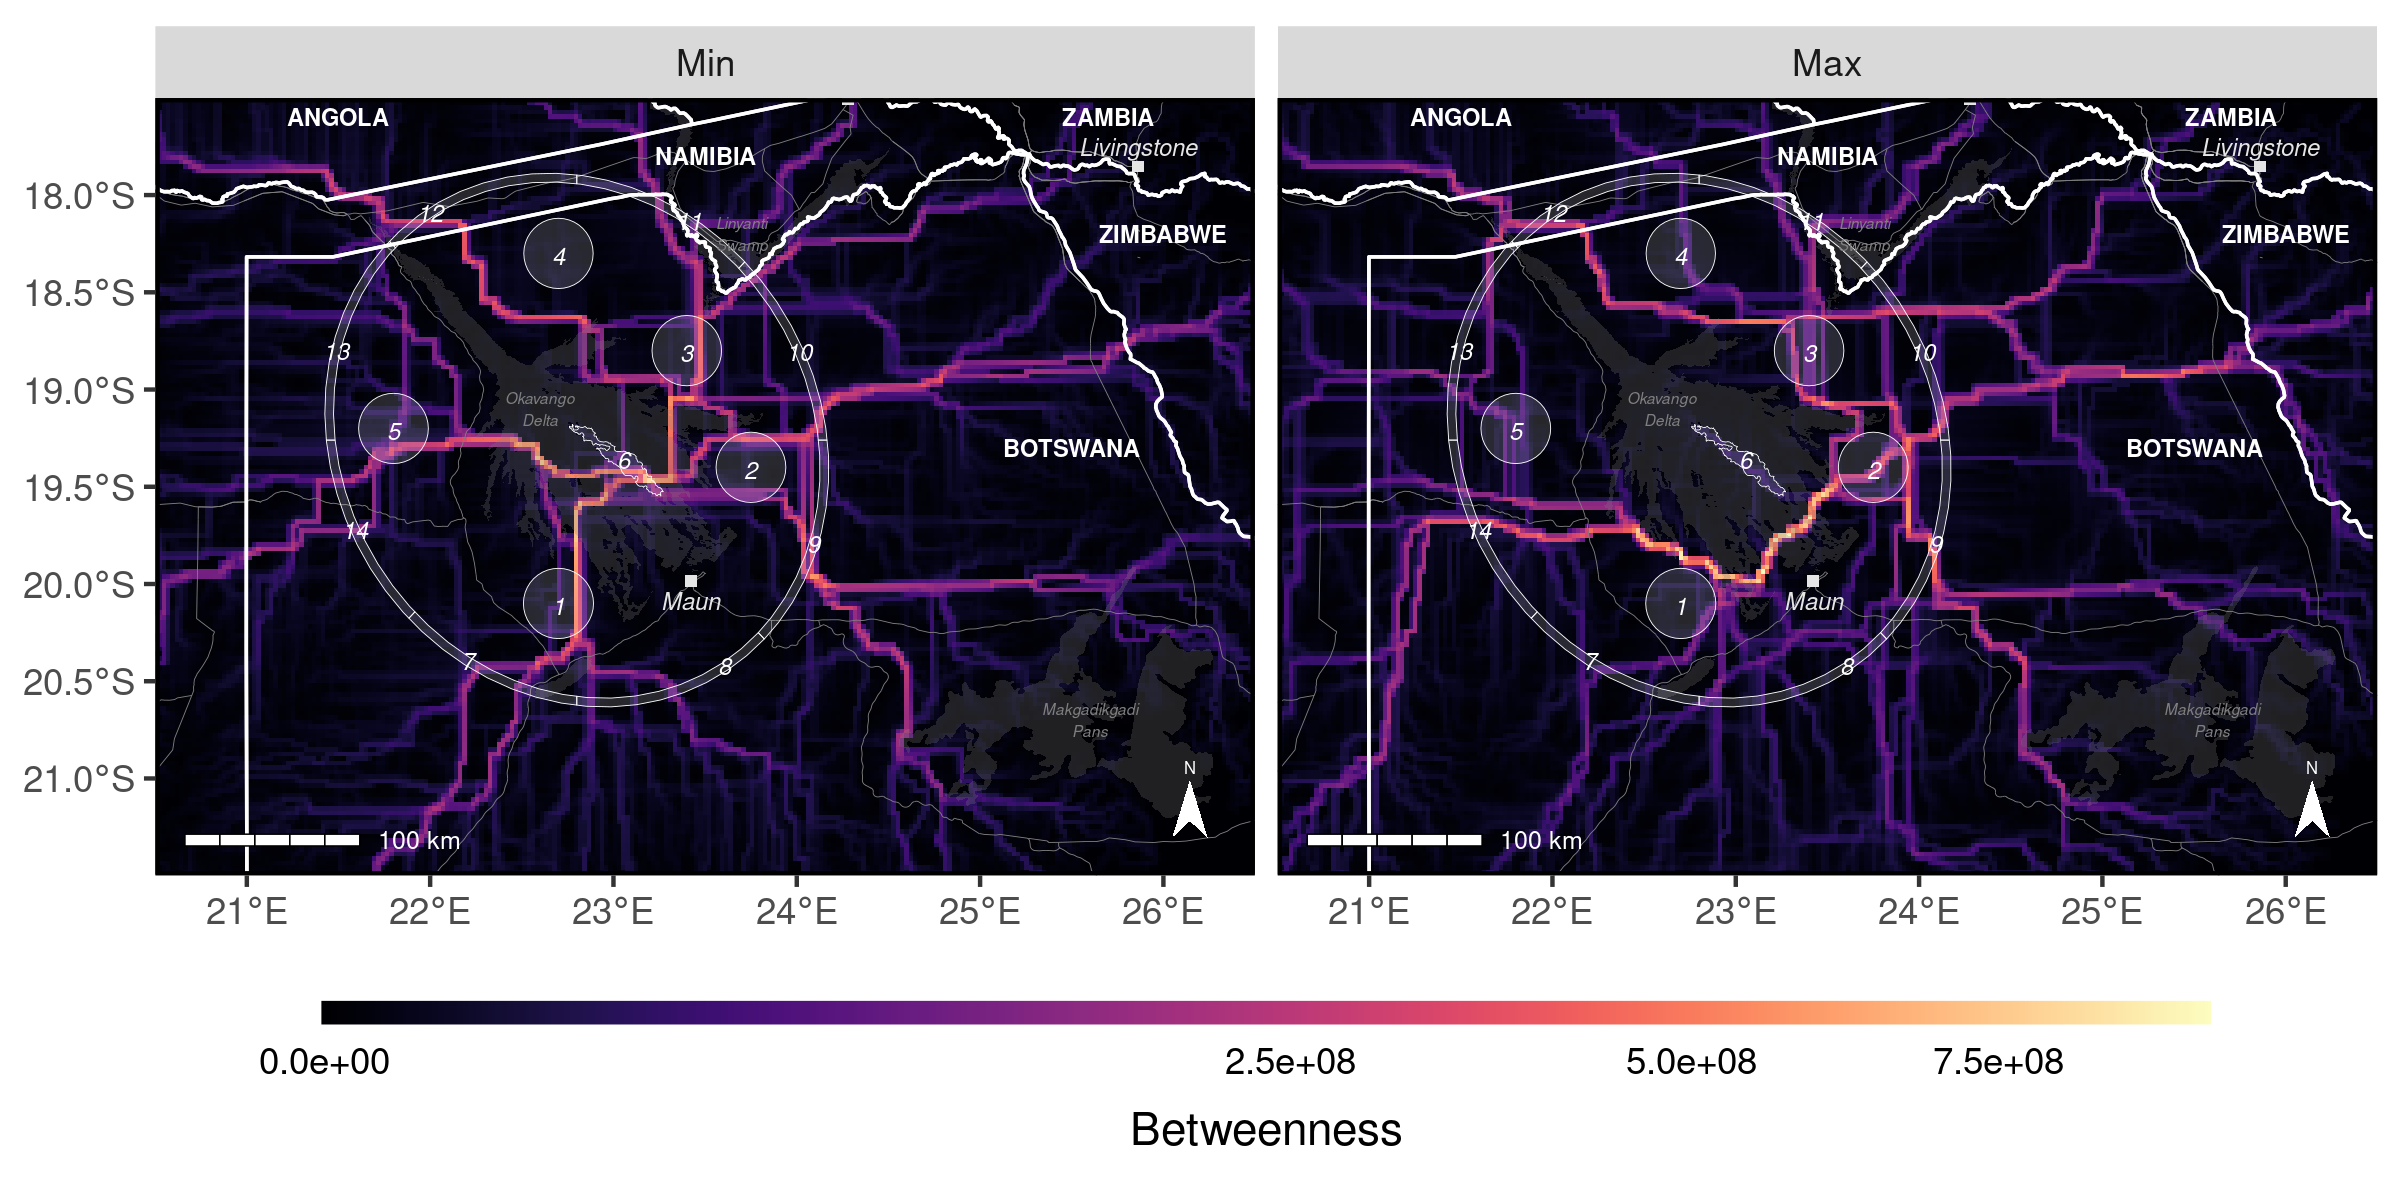
\includegraphics[width = \textwidth]{99_Betweenness.png}
  \caption{Betweenness scores highlighting potential dispersal corridors for
  both the minimum and maximum flood scenario. Areas with high betweenness
  scores (bright yellow) are used by many simulated individuals to move into
  adjacent regions and can thus be understood as critical pinch-points. Source
  areas (numbered 1-6) from which dispresers were released, and emigration zones
  (numbered 7-14) are shaded in light gray.}
  \label{Betweenness}
  \end{center}
\end{figure}

\subsection{Inter-Patch Connectivity}
Our analysis of interpatch connectivity demonstrates notable differences in
dispersal prospects and duration depending on the extent of the flood
(\Cref{IPCTable}). While $4'137$ \pm $34.60
$ simulated
dispersers reach another source area during minimum extent, only
$3626\pm36.76
$ do so during maximum extent. The
differences are particularly pronounced for individuals dispersing from or into
the source area located at the OD's center (\Cref{Interpatch}). While the area
is reached by $1325\pm32.57
$ simulated individuals
during minimum flood, only $300\pm17.30
$
dispersers arrive there during maximum flood. Furthermore, the dispersal
duration into source area six from any other source area increases from
$773\pm15.06
$ to
$920$ \pm $30.23
$. Across all simulations, the
average dispersal duration before reaching another source area increases from xx
to xx from the minimum to the maximum flood scenario. Nevertheless, connectivity
into some areas increases during maximum flooding. Emigration increased slightly
from xx to xx


For instance, while dispersers .. Additional maps highlighting differences in
inter-patch connectivty for each source area separately are provided in Appendix
SX.

\begin{figure}
  \begin{center}
  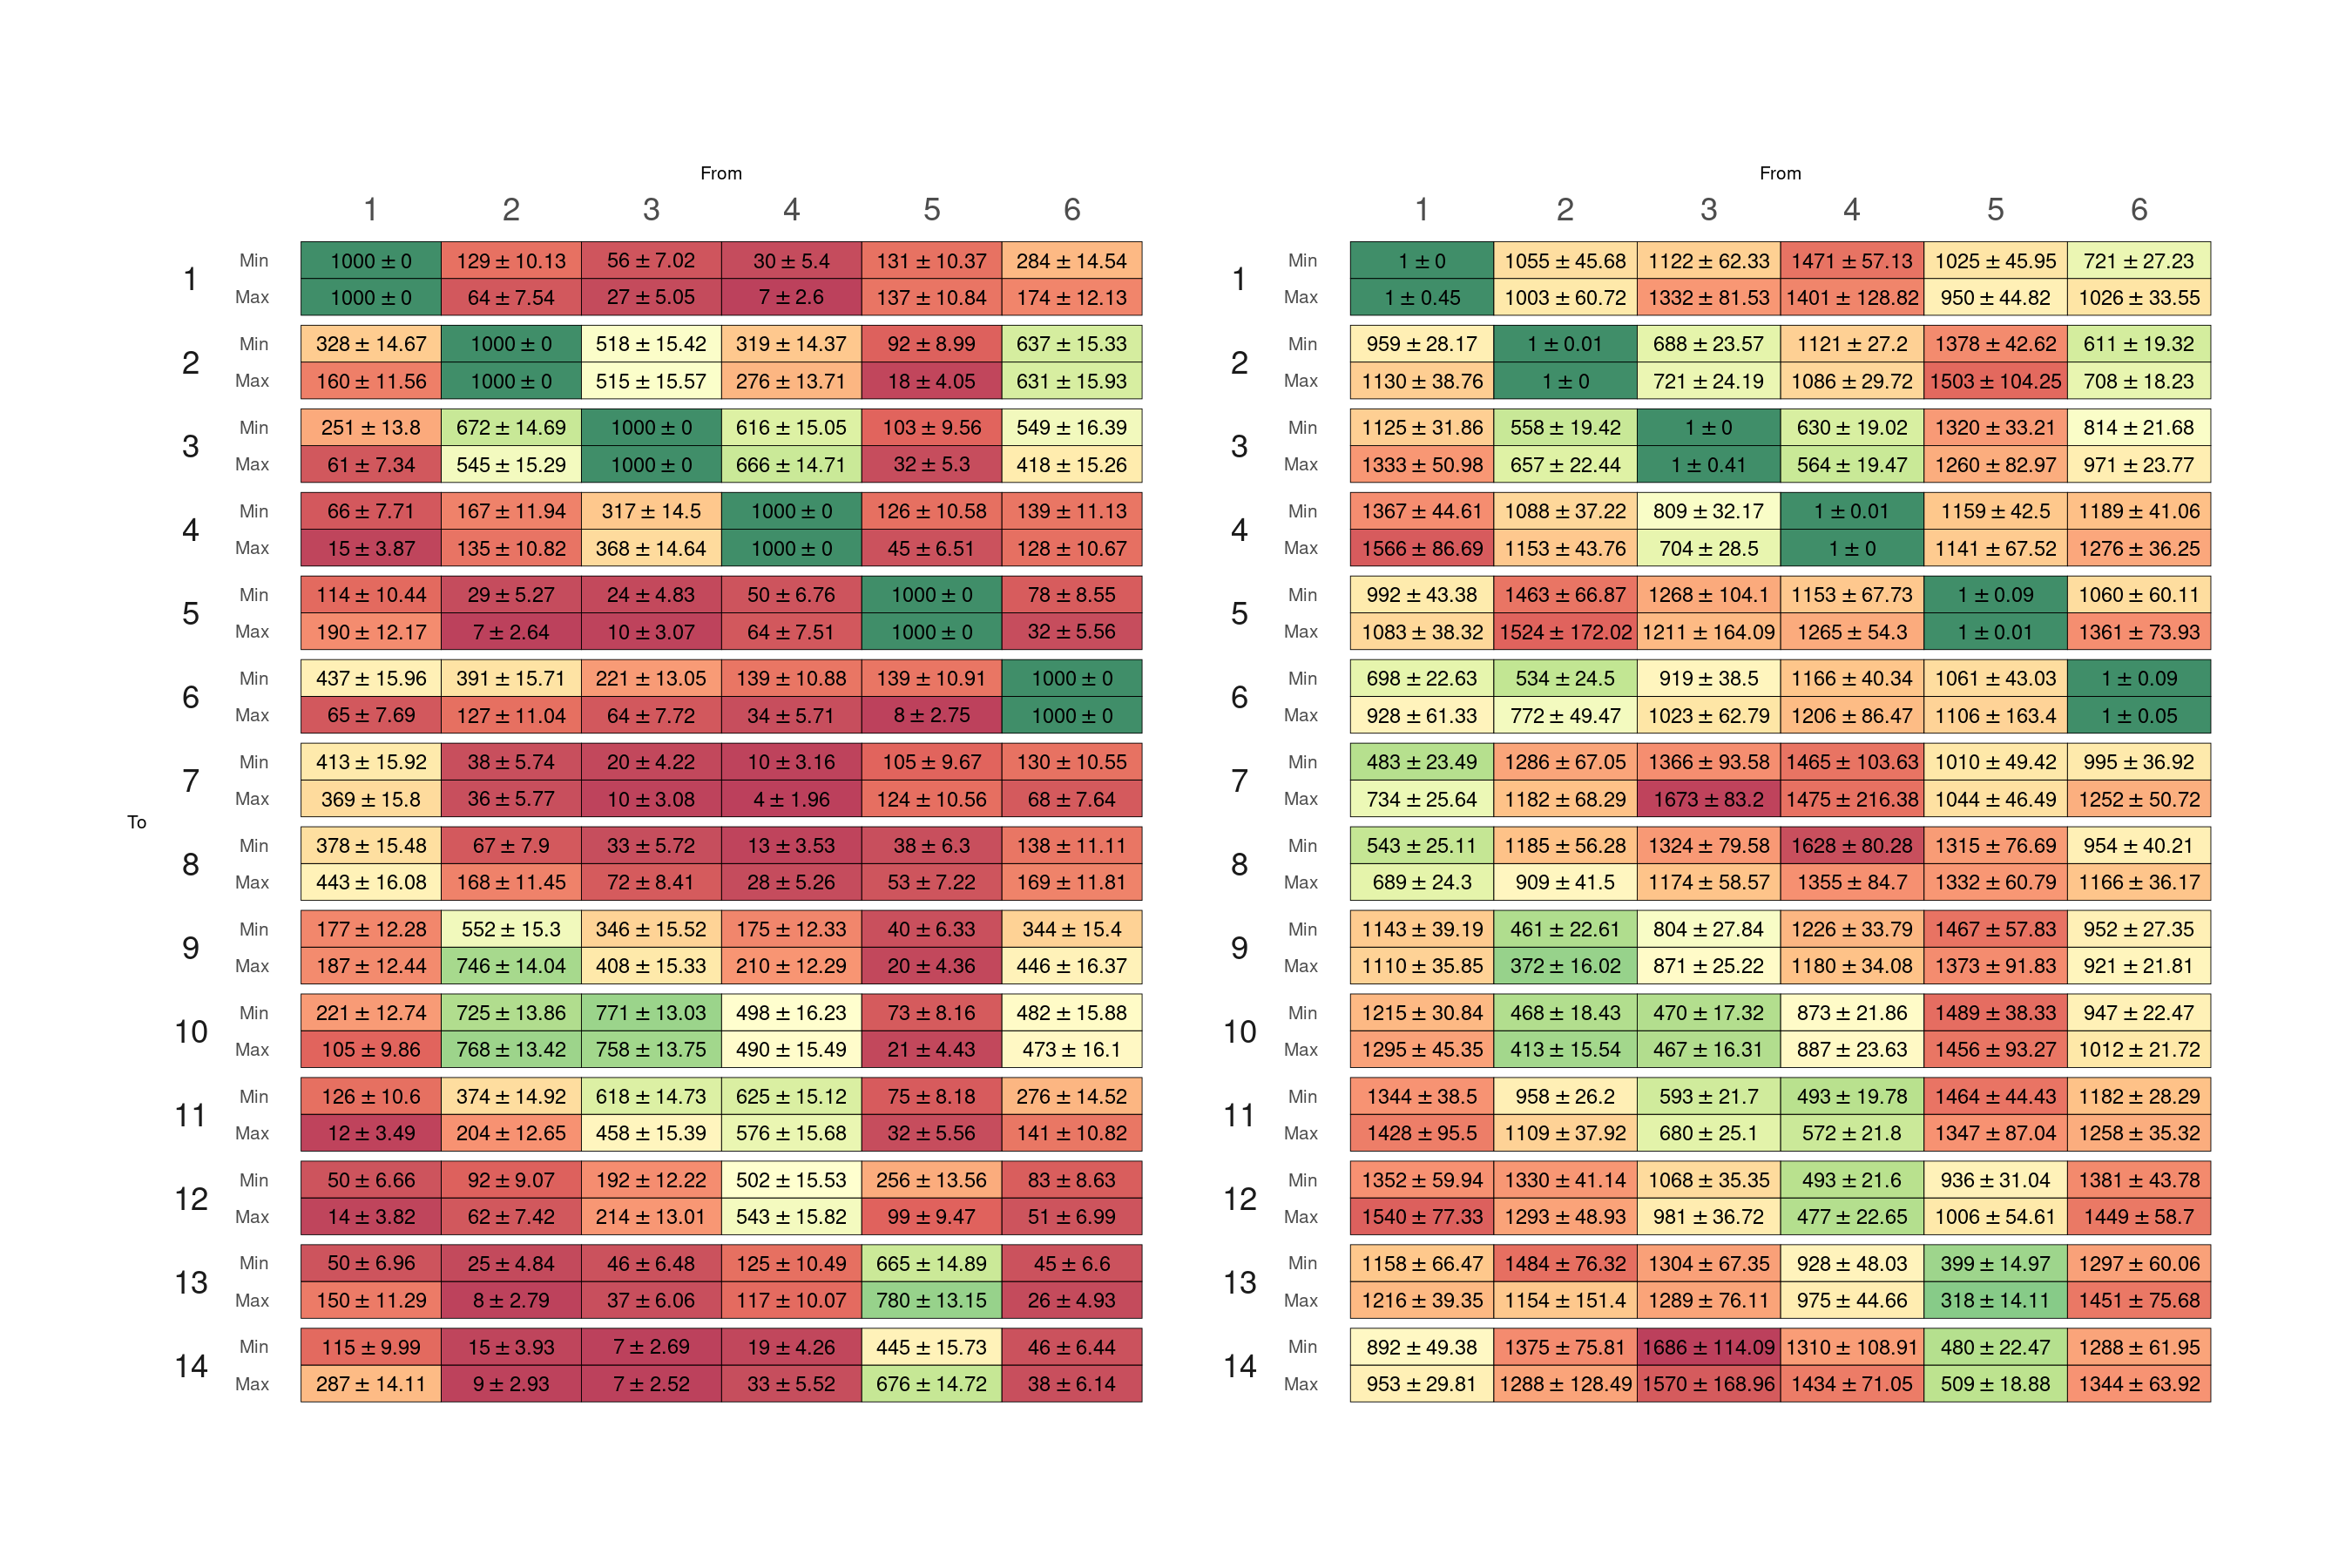
\includegraphics[width = \textwidth]{99_IPCTable.png}
  \caption{Dispersal frequency (a) and duration (b) (in steps) between source
  areas and emigration zones during minimum and maximum flood.}
  \label{IPCTable}
  \end{center}
\end{figure}

\begin{figure}
  \begin{center}
  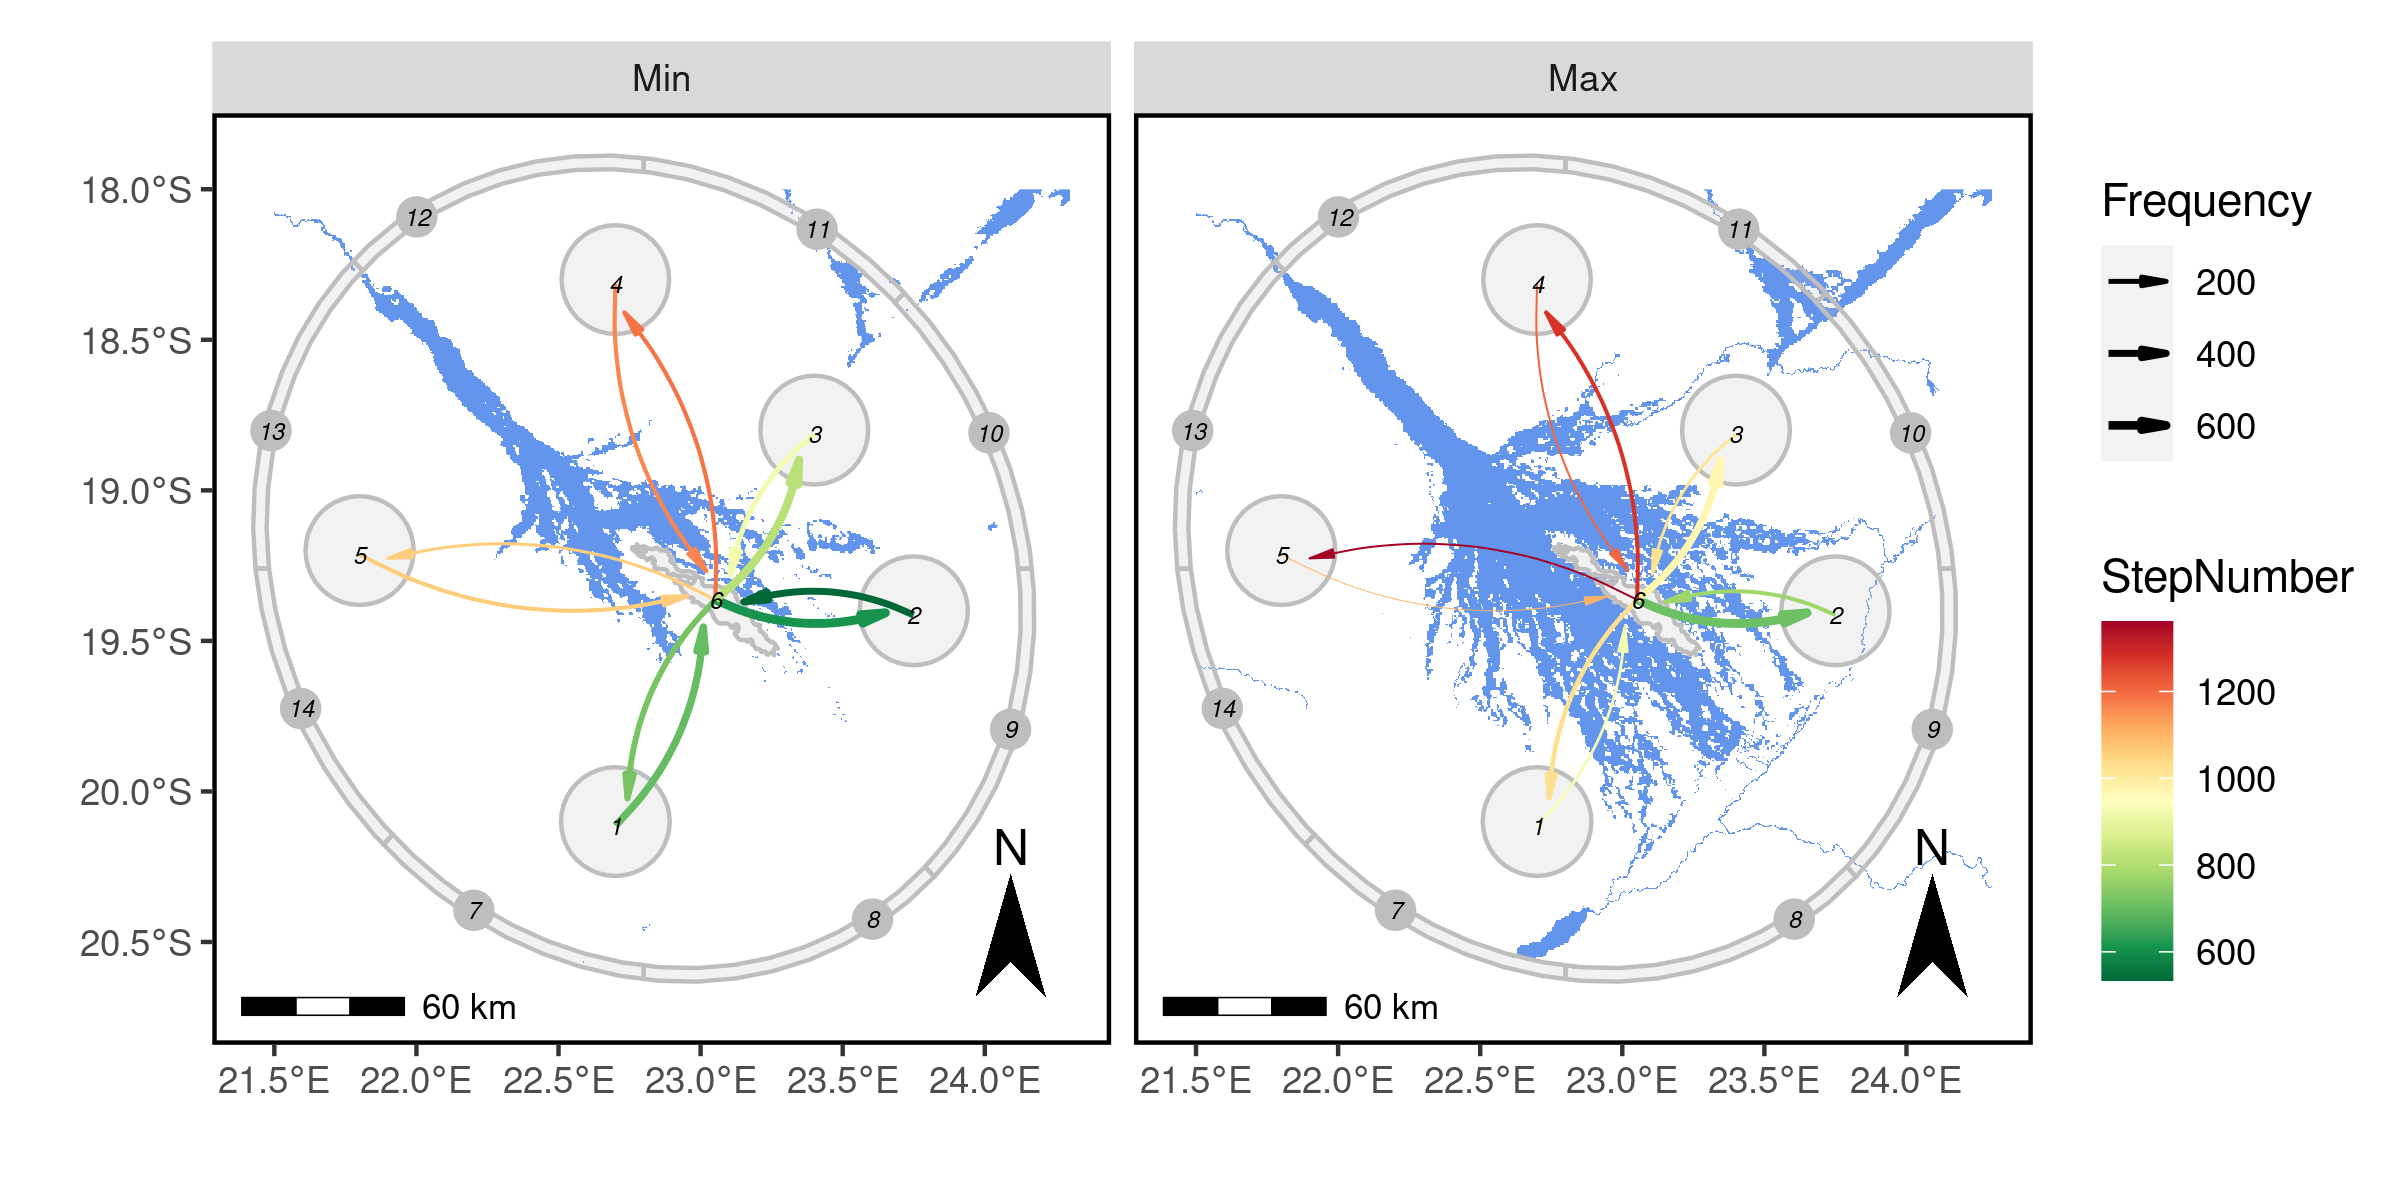
\includegraphics[width = \textwidth]{99_Interpatch.png}
  \caption{Inter-patch connectivity into and from source area number six. This
  patch experienced the most drastic reduction in connectivity in result to a
  high flood level. During minimum flood there is ample connectivity from and
  into source areas 1-3. During maximum flood, connectivity is lower and mainly
  limited to source area 2.}
  \label{Interpatch}
  \end{center}
\end{figure}

% \begin{table}

\caption{Frequency}
\centering
\resizebox{\linewidth}{!}{
\begin{tabular}[t]{rllllll}
\toprule
\multicolumn{1}{c}{} & \multicolumn{6}{c}{From} \\
\cmidrule(l{3pt}r{3pt}){2-7}
To & 1 & 2 & 3 & 4 & 5 & 6\\
\midrule
 & - & 64 $\pm$ 7.54 & 27 $\pm$ 5.05 & 7 $\pm$ 2.60 & 137 $\pm$ 10.84 & 174 $\pm$ 12.13\\

\multirow{-2}{*}{\raggedleft\arraybackslash 1} & - & 129 $\pm$ 10.13 & 56 $\pm$ 7.02 & 30 $\pm$ 5.40 & 131 $\pm$ 10.37 & 284 $\pm$ 14.54\\
\cmidrule{1-7}
 & 160 $\pm$ 11.56 & - & 515 $\pm$ 15.57 & 276 $\pm$ 13.71 & 18 $\pm$ 4.05 & 631 $\pm$ 15.93\\

\multirow{-2}{*}{\raggedleft\arraybackslash 2} & 328 $\pm$ 14.67 & - & 518 $\pm$ 15.42 & 319 $\pm$ 14.37 & 92 $\pm$ 8.99 & 637 $\pm$ 15.33\\
\cmidrule{1-7}
 & 61 $\pm$ 7.34 & 545 $\pm$ 15.29 & - & 666 $\pm$ 14.71 & 32 $\pm$ 5.30 & 418 $\pm$ 15.26\\

\multirow{-2}{*}{\raggedleft\arraybackslash 3} & 251 $\pm$ 13.80 & 672 $\pm$ 14.69 & - & 616 $\pm$ 15.05 & 103 $\pm$ 9.56 & 549 $\pm$ 16.39\\
\cmidrule{1-7}
 & 15 $\pm$ 3.87 & 135 $\pm$ 10.82 & 368 $\pm$ 14.64 & - & 45 $\pm$ 6.51 & 128 $\pm$ 10.67\\

\multirow{-2}{*}{\raggedleft\arraybackslash 4} & 66 $\pm$ 7.71 & 167 $\pm$ 11.94 & 317 $\pm$ 14.50 & - & 126 $\pm$ 10.58 & 139 $\pm$ 11.13\\
\cmidrule{1-7}
 & 190 $\pm$ 12.17 & 7 $\pm$ 2.64 & 10 $\pm$ 3.07 & 64 $\pm$ 7.51 & - & 32 $\pm$ 5.56\\

\multirow{-2}{*}{\raggedleft\arraybackslash 5} & 114 $\pm$ 10.44 & 29 $\pm$ 5.27 & 24 $\pm$ 4.83 & 50 $\pm$ 6.76 & - & 78 $\pm$ 8.55\\
\cmidrule{1-7}
 & 65 $\pm$ 7.69 & 127 $\pm$ 11.04 & 64 $\pm$ 7.72 & 34 $\pm$ 5.71 & 8 $\pm$ 2.75 & -\\

\multirow{-2}{*}{\raggedleft\arraybackslash 6} & 437 $\pm$ 15.96 & 391 $\pm$ 15.71 & 221 $\pm$ 13.05 & 139 $\pm$ 10.88 & 139 $\pm$ 10.91 & -\\
\cmidrule{1-7}
 & 369 $\pm$ 15.80 & 36 $\pm$ 5.77 & 10 $\pm$ 3.08 & 4 $\pm$ 1.96 & 124 $\pm$ 10.56 & 68 $\pm$ 7.64\\

\multirow{-2}{*}{\raggedleft\arraybackslash 7} & 413 $\pm$ 15.92 & 38 $\pm$ 5.74 & 20 $\pm$ 4.22 & 10 $\pm$ 3.16 & 105 $\pm$ 9.67 & 130 $\pm$ 10.55\\
\cmidrule{1-7}
 & 443 $\pm$ 16.08 & 168 $\pm$ 11.45 & 72 $\pm$ 8.41 & 28 $\pm$ 5.26 & 53 $\pm$ 7.22 & 169 $\pm$ 11.81\\

\multirow{-2}{*}{\raggedleft\arraybackslash 8} & 378 $\pm$ 15.48 & 67 $\pm$ 7.90 & 33 $\pm$ 5.72 & 13 $\pm$ 3.53 & 38 $\pm$ 6.30 & 138 $\pm$ 11.11\\
\cmidrule{1-7}
 & 187 $\pm$ 12.44 & 746 $\pm$ 14.04 & 408 $\pm$ 15.33 & 210 $\pm$ 12.29 & 20 $\pm$ 4.36 & 446 $\pm$ 16.37\\

\multirow{-2}{*}{\raggedleft\arraybackslash 9} & 177 $\pm$ 12.28 & 552 $\pm$ 15.30 & 346 $\pm$ 15.52 & 175 $\pm$ 12.33 & 40 $\pm$ 6.33 & 344 $\pm$ 15.40\\
\cmidrule{1-7}
 & 105 $\pm$ 9.86 & 768 $\pm$ 13.42 & 758 $\pm$ 13.75 & 490 $\pm$ 15.49 & 21 $\pm$ 4.43 & 473 $\pm$ 16.10\\

\multirow{-2}{*}{\raggedleft\arraybackslash 10} & 221 $\pm$ 12.74 & 725 $\pm$ 13.86 & 771 $\pm$ 13.03 & 498 $\pm$ 16.23 & 73 $\pm$ 8.16 & 482 $\pm$ 15.88\\
\cmidrule{1-7}
 & 12 $\pm$ 3.49 & 204 $\pm$ 12.65 & 458 $\pm$ 15.39 & 576 $\pm$ 15.68 & 32 $\pm$ 5.56 & 141 $\pm$ 10.82\\

\multirow{-2}{*}{\raggedleft\arraybackslash 11} & 126 $\pm$ 10.60 & 374 $\pm$ 14.92 & 618 $\pm$ 14.73 & 625 $\pm$ 15.12 & 75 $\pm$ 8.18 & 276 $\pm$ 14.52\\
\cmidrule{1-7}
 & 14 $\pm$ 3.82 & 62 $\pm$ 7.42 & 214 $\pm$ 13.01 & 543 $\pm$ 15.82 & 99 $\pm$ 9.47 & 51 $\pm$ 6.99\\

\multirow{-2}{*}{\raggedleft\arraybackslash 12} & 50 $\pm$ 6.66 & 92 $\pm$ 9.07 & 192 $\pm$ 12.22 & 502 $\pm$ 15.53 & 256 $\pm$ 13.56 & 83 $\pm$ 8.63\\
\cmidrule{1-7}
 & 150 $\pm$ 11.29 & 8 $\pm$ 2.79 & 37 $\pm$ 6.06 & 117 $\pm$ 10.07 & 780 $\pm$ 13.15 & 26 $\pm$ 4.93\\

\multirow{-2}{*}{\raggedleft\arraybackslash 13} & 50 $\pm$ 6.96 & 25 $\pm$ 4.84 & 46 $\pm$ 6.48 & 125 $\pm$ 10.49 & 665 $\pm$ 14.89 & 45 $\pm$ 6.60\\
\cmidrule{1-7}
 & 287 $\pm$ 14.11 & 9 $\pm$ 2.93 & 7 $\pm$ 2.52 & 33 $\pm$ 5.52 & 676 $\pm$ 14.72 & 38 $\pm$ 6.14\\

\multirow{-2}{*}{\raggedleft\arraybackslash 14} & 115 $\pm$ 9.99 & 15 $\pm$ 3.93 & 7 $\pm$ 2.69 & 19 $\pm$ 4.26 & 445 $\pm$ 15.73 & 46 $\pm$ 6.44\\
\bottomrule
\end{tabular}}
\end{table}

% \begin{table}

\caption{Duration}
\centering
\resizebox{\linewidth}{!}{
\begin{tabular}[t]{rllllll}
\toprule
\multicolumn{1}{c}{} & \multicolumn{6}{c}{From} \\
\cmidrule(l{3pt}r{3pt}){2-7}
To & 1 & 2 & 3 & 4 & 5 & 6\\
\midrule
 & - & 1052 $\pm$ 45.57 & 1123 $\pm$ 62.35 & 1475 $\pm$ 59.49 & 1024 $\pm$ 44.65 & 721 $\pm$ 28.59\\

\multirow{-2}{*}{\raggedleft\arraybackslash 1} & - & 1010 $\pm$ 59.36 & 1329 $\pm$ 79.10 & 1411 $\pm$ 124.88 & 949 $\pm$ 44.16 & 1027 $\pm$ 33.84\\
\cmidrule{1-7}
 & 960 $\pm$ 28.44 & - & 688 $\pm$ 22.56 & 1120 $\pm$ 26.52 & 1378 $\pm$ 43.10 & 611 $\pm$ 19.05\\

\multirow{-2}{*}{\raggedleft\arraybackslash 2} & 1128 $\pm$ 39.18 & - & 723 $\pm$ 23.68 & 1086 $\pm$ 30.07 & 1506 $\pm$ 101.35 & 709 $\pm$ 19.28\\
\cmidrule{1-7}
 & 1125 $\pm$ 32.17 & 558 $\pm$ 19.47 & - & 629 $\pm$ 18.99 & 1318 $\pm$ 35.16 & 814 $\pm$ 22.05\\

\multirow{-2}{*}{\raggedleft\arraybackslash 3} & 1330 $\pm$ 51.15 & 658 $\pm$ 21.34 & - & 564 $\pm$ 19.18 & 1263 $\pm$ 86.09 & 972 $\pm$ 24.72\\
\cmidrule{1-7}
 & 1369 $\pm$ 45.60 & 1085 $\pm$ 38.00 & 807 $\pm$ 31.14 & - & 1161 $\pm$ 42.09 & 1188 $\pm$ 40.24\\

\multirow{-2}{*}{\raggedleft\arraybackslash 4} & 1568 $\pm$ 88.27 & 1151 $\pm$ 43.04 & 704 $\pm$ 29.70 & - & 1140 $\pm$ 66.77 & 1275 $\pm$ 37.76\\
\cmidrule{1-7}
 & 991 $\pm$ 45.90 & 1465 $\pm$ 69.63 & 1262 $\pm$ 106.51 & 1153 $\pm$ 70.15 & - & 1065 $\pm$ 57.26\\

\multirow{-2}{*}{\raggedleft\arraybackslash 5} & 1083 $\pm$ 38.26 & 1526 $\pm$ 169.88 & 1216 $\pm$ 160.94 & 1269 $\pm$ 50.48 & - & 1359 $\pm$ 71.28\\
\cmidrule{1-7}
 & 696 $\pm$ 23.21 & 535 $\pm$ 25.03 & 921 $\pm$ 39.88 & 1165 $\pm$ 41.97 & 1064 $\pm$ 42.00 & -\\

\multirow{-2}{*}{\raggedleft\arraybackslash 6} & 928 $\pm$ 59.98 & 777 $\pm$ 50.21 & 1022 $\pm$ 62.82 & 1204 $\pm$ 83.77 & 1113 $\pm$ 162.42 & -\\
\cmidrule{1-7}
 & 483 $\pm$ 23.02 & 1290 $\pm$ 65.55 & 1361 $\pm$ 93.87 & 1463 $\pm$ 106.88 & 1011 $\pm$ 50.72 & 995 $\pm$ 37.14\\

\multirow{-2}{*}{\raggedleft\arraybackslash 7} & 734 $\pm$ 26.74 & 1180 $\pm$ 68.81 & 1671 $\pm$ 84.10 & 1486 $\pm$ 216.02 & 1046 $\pm$ 49.97 & 1253 $\pm$ 49.81\\
\cmidrule{1-7}
 & 543 $\pm$ 24.93 & 1188 $\pm$ 58.61 & 1326 $\pm$ 76.33 & 1627 $\pm$ 80.53 & 1312 $\pm$ 76.45 & 953 $\pm$ 41.08\\

\multirow{-2}{*}{\raggedleft\arraybackslash 8} & 688 $\pm$ 23.74 & 908 $\pm$ 41.43 & 1177 $\pm$ 56.84 & 1352 $\pm$ 79.76 & 1329 $\pm$ 55.66 & 1167 $\pm$ 37.50\\
\cmidrule{1-7}
 & 1145 $\pm$ 38.84 & 462 $\pm$ 21.34 & 805 $\pm$ 27.76 & 1225 $\pm$ 35.91 & 1462 $\pm$ 59.73 & 950 $\pm$ 25.88\\

\multirow{-2}{*}{\raggedleft\arraybackslash 9} & 1109 $\pm$ 34.28 & 372 $\pm$ 16.47 & 872 $\pm$ 24.91 & 1179 $\pm$ 34.64 & 1376 $\pm$ 89.62 & 921 $\pm$ 22.52\\
\cmidrule{1-7}
 & 1214 $\pm$ 30.66 & 468 $\pm$ 17.95 & 471 $\pm$ 17.71 & 872 $\pm$ 22.31 & 1489 $\pm$ 40.00 & 946 $\pm$ 22.06\\

\multirow{-2}{*}{\raggedleft\arraybackslash 10} & 1294 $\pm$ 45.11 & 413 $\pm$ 15.31 & 467 $\pm$ 16.58 & 886 $\pm$ 22.69 & 1456 $\pm$ 92.16 & 1014 $\pm$ 22.45\\
\cmidrule{1-7}
 & 1345 $\pm$ 39.71 & 959 $\pm$ 27.15 & 592 $\pm$ 21.91 & 493 $\pm$ 19.92 & 1463 $\pm$ 43.67 & 1181 $\pm$ 28.88\\

\multirow{-2}{*}{\raggedleft\arraybackslash 11} & 1425 $\pm$ 102.10 & 1109 $\pm$ 36.18 & 681 $\pm$ 25.66 & 572 $\pm$ 21.75 & 1346 $\pm$ 85.45 & 1255 $\pm$ 35.85\\
\cmidrule{1-7}
 & 1359 $\pm$ 61.03 & 1327 $\pm$ 41.72 & 1066 $\pm$ 34.40 & 493 $\pm$ 20.75 & 937 $\pm$ 30.63 & 1382 $\pm$ 42.85\\

\multirow{-2}{*}{\raggedleft\arraybackslash 12} & 1534 $\pm$ 78.37 & 1292 $\pm$ 51.25 & 981 $\pm$ 34.48 & 478 $\pm$ 22.21 & 1005 $\pm$ 56.52 & 1445 $\pm$ 57.51\\
\cmidrule{1-7}
 & 1160 $\pm$ 66.27 & 1479 $\pm$ 76.43 & 1300 $\pm$ 66.24 & 927 $\pm$ 49.65 & 399 $\pm$ 15.63 & 1302 $\pm$ 59.59\\

\multirow{-2}{*}{\raggedleft\arraybackslash 13} & 1219 $\pm$ 40.97 & 1148 $\pm$ 149.50 & 1289 $\pm$ 80.28 & 975 $\pm$ 49.38 & 319 $\pm$ 14.14 & 1453 $\pm$ 73.18\\
\cmidrule{1-7}
 & 893 $\pm$ 50.08 & 1376 $\pm$ 78.19 & 1684 $\pm$ 112.78 & 1304 $\pm$ 115.43 & 480 $\pm$ 22.25 & 1293 $\pm$ 60.16\\

\multirow{-2}{*}{\raggedleft\arraybackslash 14} & 954 $\pm$ 30.69 & 1287 $\pm$ 132.10 & 1569 $\pm$ 175.42 & 1435 $\pm$ 71.93 & 509 $\pm$ 19.21 & 1342 $\pm$ 60.78\\
\bottomrule
\end{tabular}}
\end{table}

% \begin{table}

\caption{Duration}
\centering
\resizebox{\linewidth}{!}{
\begin{tabular}[t]{rllllllllllll}
\toprule
\multicolumn{1}{c}{} & \multicolumn{6}{c}{Frequency} & \multicolumn{6}{c}{Duration} \\
\cmidrule(l{3pt}r{3pt}){2-7} \cmidrule(l{3pt}r{3pt}){8-13}
\multicolumn{1}{c}{} & \multicolumn{12}{c}{From} \\
\cmidrule(l{3pt}r{3pt}){2-13}
To & 1 & 2 & 3 & 4 & 5 & 6 & 1 & 2 & 3 & 4 & 5 & 6\\
\midrule
 & - & 129 $\pm$ 10.13 & 56 $\pm$ 7.02 & 30 $\pm$ 5.40 & 131 $\pm$ 10.37 & 284 $\pm$ 14.54 & - & 1055 $\pm$ 45.68 & 1122 $\pm$ 62.33 & 1471 $\pm$ 57.13 & 1025 $\pm$ 45.95 & 721 $\pm$ 27.23\\

\multirow{-2}{*}{\raggedleft\arraybackslash 1} & - & 64 $\pm$ 7.54 & 27 $\pm$ 5.05 & 7 $\pm$ 2.60 & 137 $\pm$ 10.84 & 174 $\pm$ 12.13 & - & 1003 $\pm$ 60.72 & 1332 $\pm$ 81.53 & 1401 $\pm$ 128.82 & 950 $\pm$ 44.82 & 1026 $\pm$ 33.55\\
\cmidrule{1-13}
 & 328 $\pm$ 14.67 & - & 518 $\pm$ 15.42 & 319 $\pm$ 14.37 & 92 $\pm$ 8.99 & 637 $\pm$ 15.33 & 959 $\pm$ 28.17 & - & 688 $\pm$ 23.57 & 1121 $\pm$ 27.20 & 1378 $\pm$ 42.62 & 611 $\pm$ 19.32\\

\multirow{-2}{*}{\raggedleft\arraybackslash 2} & 160 $\pm$ 11.56 & - & 515 $\pm$ 15.57 & 276 $\pm$ 13.71 & 18 $\pm$ 4.05 & 631 $\pm$ 15.93 & 1130 $\pm$ 38.76 & - & 721 $\pm$ 24.19 & 1086 $\pm$ 29.72 & 1503 $\pm$ 104.25 & 708 $\pm$ 18.23\\
\cmidrule{1-13}
 & 251 $\pm$ 13.80 & 672 $\pm$ 14.69 & - & 616 $\pm$ 15.05 & 103 $\pm$ 9.56 & 549 $\pm$ 16.39 & 1125 $\pm$ 31.86 & 558 $\pm$ 19.42 & - & 630 $\pm$ 19.02 & 1320 $\pm$ 33.21 & 814 $\pm$ 21.68\\

\multirow{-2}{*}{\raggedleft\arraybackslash 3} & 61 $\pm$ 7.34 & 545 $\pm$ 15.29 & - & 666 $\pm$ 14.71 & 32 $\pm$ 5.30 & 418 $\pm$ 15.26 & 1333 $\pm$ 50.98 & 657 $\pm$ 22.44 & - & 564 $\pm$ 19.47 & 1260 $\pm$ 82.97 & 971 $\pm$ 23.77\\
\cmidrule{1-13}
 & 66 $\pm$ 7.71 & 167 $\pm$ 11.94 & 317 $\pm$ 14.50 & - & 126 $\pm$ 10.58 & 139 $\pm$ 11.13 & 1367 $\pm$ 44.61 & 1088 $\pm$ 37.22 & 809 $\pm$ 32.17 & - & 1159 $\pm$ 42.50 & 1189 $\pm$ 41.06\\

\multirow{-2}{*}{\raggedleft\arraybackslash 4} & 15 $\pm$ 3.87 & 135 $\pm$ 10.82 & 368 $\pm$ 14.64 & - & 45 $\pm$ 6.51 & 128 $\pm$ 10.67 & 1566 $\pm$ 86.69 & 1153 $\pm$ 43.76 & 704 $\pm$ 28.50 & - & 1141 $\pm$ 67.52 & 1276 $\pm$ 36.25\\
\cmidrule{1-13}
 & 114 $\pm$ 10.44 & 29 $\pm$ 5.27 & 24 $\pm$ 4.83 & 50 $\pm$ 6.76 & - & 78 $\pm$ 8.55 & 992 $\pm$ 43.38 & 1463 $\pm$ 66.87 & 1268 $\pm$ 104.10 & 1153 $\pm$ 67.73 & - & 1060 $\pm$ 60.11\\

\multirow{-2}{*}{\raggedleft\arraybackslash 5} & 190 $\pm$ 12.17 & 7 $\pm$ 2.64 & 10 $\pm$ 3.07 & 64 $\pm$ 7.51 & - & 32 $\pm$ 5.56 & 1083 $\pm$ 38.32 & 1524 $\pm$ 172.02 & 1211 $\pm$ 164.09 & 1265 $\pm$ 54.30 & - & 1361 $\pm$ 73.93\\
\cmidrule{1-13}
 & 437 $\pm$ 15.96 & 391 $\pm$ 15.71 & 221 $\pm$ 13.05 & 139 $\pm$ 10.88 & 139 $\pm$ 10.91 & - & 698 $\pm$ 22.63 & 534 $\pm$ 24.50 & 919 $\pm$ 38.50 & 1166 $\pm$ 40.34 & 1061 $\pm$ 43.03 & -\\

\multirow{-2}{*}{\raggedleft\arraybackslash 6} & 65 $\pm$ 7.69 & 127 $\pm$ 11.04 & 64 $\pm$ 7.72 & 34 $\pm$ 5.71 & 8 $\pm$ 2.75 & - & 928 $\pm$ 61.33 & 772 $\pm$ 49.47 & 1023 $\pm$ 62.79 & 1206 $\pm$ 86.47 & 1106 $\pm$ 163.40 & -\\
\cmidrule{1-13}
 & 413 $\pm$ 15.92 & 38 $\pm$ 5.74 & 20 $\pm$ 4.22 & 10 $\pm$ 3.16 & 105 $\pm$ 9.67 & 130 $\pm$ 10.55 & 483 $\pm$ 23.49 & 1286 $\pm$ 67.05 & 1366 $\pm$ 93.58 & 1465 $\pm$ 103.63 & 1010 $\pm$ 49.42 & 995 $\pm$ 36.92\\

\multirow{-2}{*}{\raggedleft\arraybackslash 7} & 369 $\pm$ 15.80 & 36 $\pm$ 5.77 & 10 $\pm$ 3.08 & 4 $\pm$ 1.96 & 124 $\pm$ 10.56 & 68 $\pm$ 7.64 & 734 $\pm$ 25.64 & 1182 $\pm$ 68.29 & 1673 $\pm$ 83.20 & 1475 $\pm$ 216.38 & 1044 $\pm$ 46.49 & 1252 $\pm$ 50.72\\
\cmidrule{1-13}
 & 378 $\pm$ 15.48 & 67 $\pm$ 7.90 & 33 $\pm$ 5.72 & 13 $\pm$ 3.53 & 38 $\pm$ 6.30 & 138 $\pm$ 11.11 & 543 $\pm$ 25.11 & 1185 $\pm$ 56.28 & 1324 $\pm$ 79.58 & 1628 $\pm$ 80.28 & 1315 $\pm$ 76.69 & 954 $\pm$ 40.21\\

\multirow{-2}{*}{\raggedleft\arraybackslash 8} & 443 $\pm$ 16.08 & 168 $\pm$ 11.45 & 72 $\pm$ 8.41 & 28 $\pm$ 5.26 & 53 $\pm$ 7.22 & 169 $\pm$ 11.81 & 689 $\pm$ 24.30 & 909 $\pm$ 41.50 & 1174 $\pm$ 58.57 & 1355 $\pm$ 84.70 & 1332 $\pm$ 60.79 & 1166 $\pm$ 36.17\\
\cmidrule{1-13}
 & 177 $\pm$ 12.28 & 552 $\pm$ 15.30 & 346 $\pm$ 15.52 & 175 $\pm$ 12.33 & 40 $\pm$ 6.33 & 344 $\pm$ 15.40 & 1143 $\pm$ 39.19 & 461 $\pm$ 22.61 & 804 $\pm$ 27.84 & 1226 $\pm$ 33.79 & 1467 $\pm$ 57.83 & 952 $\pm$ 27.35\\

\multirow{-2}{*}{\raggedleft\arraybackslash 9} & 187 $\pm$ 12.44 & 746 $\pm$ 14.04 & 408 $\pm$ 15.33 & 210 $\pm$ 12.29 & 20 $\pm$ 4.36 & 446 $\pm$ 16.37 & 1110 $\pm$ 35.85 & 372 $\pm$ 16.02 & 871 $\pm$ 25.22 & 1180 $\pm$ 34.08 & 1373 $\pm$ 91.83 & 921 $\pm$ 21.81\\
\cmidrule{1-13}
 & 221 $\pm$ 12.74 & 725 $\pm$ 13.86 & 771 $\pm$ 13.03 & 498 $\pm$ 16.23 & 73 $\pm$ 8.16 & 482 $\pm$ 15.88 & 1215 $\pm$ 30.84 & 468 $\pm$ 18.43 & 470 $\pm$ 17.32 & 873 $\pm$ 21.86 & 1489 $\pm$ 38.33 & 947 $\pm$ 22.47\\

\multirow{-2}{*}{\raggedleft\arraybackslash 10} & 105 $\pm$ 9.86 & 768 $\pm$ 13.42 & 758 $\pm$ 13.75 & 490 $\pm$ 15.49 & 21 $\pm$ 4.43 & 473 $\pm$ 16.10 & 1295 $\pm$ 45.35 & 413 $\pm$ 15.54 & 467 $\pm$ 16.31 & 887 $\pm$ 23.63 & 1456 $\pm$ 93.27 & 1012 $\pm$ 21.72\\
\cmidrule{1-13}
 & 126 $\pm$ 10.60 & 374 $\pm$ 14.92 & 618 $\pm$ 14.73 & 625 $\pm$ 15.12 & 75 $\pm$ 8.18 & 276 $\pm$ 14.52 & 1344 $\pm$ 38.50 & 958 $\pm$ 26.20 & 593 $\pm$ 21.70 & 493 $\pm$ 19.78 & 1464 $\pm$ 44.43 & 1182 $\pm$ 28.29\\

\multirow{-2}{*}{\raggedleft\arraybackslash 11} & 12 $\pm$ 3.49 & 204 $\pm$ 12.65 & 458 $\pm$ 15.39 & 576 $\pm$ 15.68 & 32 $\pm$ 5.56 & 141 $\pm$ 10.82 & 1428 $\pm$ 95.50 & 1109 $\pm$ 37.92 & 680 $\pm$ 25.10 & 572 $\pm$ 21.80 & 1347 $\pm$ 87.04 & 1258 $\pm$ 35.32\\
\cmidrule{1-13}
 & 50 $\pm$ 6.66 & 92 $\pm$ 9.07 & 192 $\pm$ 12.22 & 502 $\pm$ 15.53 & 256 $\pm$ 13.56 & 83 $\pm$ 8.63 & 1352 $\pm$ 59.94 & 1330 $\pm$ 41.14 & 1068 $\pm$ 35.35 & 493 $\pm$ 21.60 & 936 $\pm$ 31.04 & 1381 $\pm$ 43.78\\

\multirow{-2}{*}{\raggedleft\arraybackslash 12} & 14 $\pm$ 3.82 & 62 $\pm$ 7.42 & 214 $\pm$ 13.01 & 543 $\pm$ 15.82 & 99 $\pm$ 9.47 & 51 $\pm$ 6.99 & 1540 $\pm$ 77.33 & 1293 $\pm$ 48.93 & 981 $\pm$ 36.72 & 477 $\pm$ 22.65 & 1006 $\pm$ 54.61 & 1449 $\pm$ 58.70\\
\cmidrule{1-13}
 & 50 $\pm$ 6.96 & 25 $\pm$ 4.84 & 46 $\pm$ 6.48 & 125 $\pm$ 10.49 & 665 $\pm$ 14.89 & 45 $\pm$ 6.60 & 1158 $\pm$ 66.47 & 1484 $\pm$ 76.32 & 1304 $\pm$ 67.35 & 928 $\pm$ 48.03 & 399 $\pm$ 14.97 & 1297 $\pm$ 60.06\\

\multirow{-2}{*}{\raggedleft\arraybackslash 13} & 150 $\pm$ 11.29 & 8 $\pm$ 2.79 & 37 $\pm$ 6.06 & 117 $\pm$ 10.07 & 780 $\pm$ 13.15 & 26 $\pm$ 4.93 & 1216 $\pm$ 39.35 & 1154 $\pm$ 151.40 & 1289 $\pm$ 76.11 & 975 $\pm$ 44.66 & 318 $\pm$ 14.11 & 1451 $\pm$ 75.68\\
\cmidrule{1-13}
 & 115 $\pm$ 9.99 & 15 $\pm$ 3.93 & 7 $\pm$ 2.69 & 19 $\pm$ 4.26 & 445 $\pm$ 15.73 & 46 $\pm$ 6.44 & 892 $\pm$ 49.38 & 1375 $\pm$ 75.81 & 1686 $\pm$ 114.09 & 1310 $\pm$ 108.91 & 480 $\pm$ 22.47 & 1288 $\pm$ 61.95\\

\multirow{-2}{*}{\raggedleft\arraybackslash 14} & 287 $\pm$ 14.11 & 9 $\pm$ 2.93 & 7 $\pm$ 2.52 & 33 $\pm$ 5.52 & 676 $\pm$ 14.72 & 38 $\pm$ 6.14 & 953 $\pm$ 29.81 & 1288 $\pm$ 128.49 & 1570 $\pm$ 168.96 & 1434 $\pm$ 71.05 & 509 $\pm$ 18.88 & 1344 $\pm$ 63.92\\
\bottomrule
\end{tabular}}
\end{table}


\section{Discussion}
According to our simulations, the propensity to move between the eastern and
western part of the delta is much lower during maximum extent. This is mainly
due to the flood-waters and the city of Maun acting as dispersal barriers.
During maximum extent, the floodwaters of the delta close a gap between the
delta and Maun that otherwise would serve as dispersal corridor. Anecdotal
evidence supports this hypothesis, for the only dispersing individuals recorded
to move from the eastern to the western part of the delta moved at times of low
flood. In line with this, it appears that a large flood extent pushes dispersing
individuals to move closer to human inhabited areas such as the village of Maun.

Predicting how climate change will impact the dispersal ability of AWDs is
challenging for multiple reasons. First of all, predicting the flooding patterns
of the OD under climate change is merely impossible due to the complex feedbacks
between surface-temperature, soil conditions, precipitation patterns and the
associated changes in vegetation. Second, the delta is not only prone to changes
in environmental conditions, but also to changes in anthropogenic use of the
inflowing water. Finally, it is unclear how AWDs, in fact, how any
species, will cope with environmental change due to global warming. Even though
some studies predict that AWD populations are likely to decline under increasing
temperatures, these studies fail to account for the behavioral plasticity of
their focal species. AWDs respiratory system, for instance, has evolved as a
perfect adaptation to high temperatures and AWDs may, in fact, profit from a
comparative advantage (cite an economist) over their competitors and prey under
rising temperatures. Although the theory of comparative advantages is a
fundamental concept in economics, it has yet to find its way into ecological
studies.

\cite{Murray-Hudson.2006} predicted that increased temperatures, additional human
abstractions, and reduced river flows might lead to a ``Delta dying'' and that
the impact of climate will be much more pronounced than the impact of
anthropogenic water use.

Although local rainfalls in Botswana are expected to increase in terms of
intensity, simulations show that the length of the rainy season will decline,
more than offsetting the incline in precipitation \cite{Akinyemi.2019}.

We studied a population of African wild dogs that resides in a natural
environment with little human influence. This is only representative for a small
share of the extant wild dog populations, as most individuals reside in areas
that are prone to substantial edge effects. For these populations, the benefit
of dispersal is disputed, as dispersal under high anthropogenic mortality may
lead to a net-loss of individuals \citep{Leigh.2012}.

We assessed the implications of environmental change on the dispersal prospects,
yet we did not consider how changing conditions alter dispersal propensity.

According to our simulations, dispersers are able to cover larger distances
during periods of low flood. This finding is little surprising, considering that
inundated areas act as dispersal barriers and force dispersers to detour and
circumvent water-covered areas. However, it still leads to an interesting
hypothesis. Previous studies have shown that the euclidean dispersal distance of
female coalitions is larger than that of male coalitions. This has led to ...
However, demographic analyses have also revealed that female offspring tend to
emigrate from their pack at younger ages and earlier in the year, when
floodwaters are still at a relatively low level (Behr). It is thus conceivable
that the sex-differences in reported dispersal distances is mainly a consequence
of environmental conditions during dispersal, rather than owed to physiological
differences between sexes.

While our analysis marks an important step into incorporating environmental
change into studies of connectivity, there are several critical additions that
should be considered in the future. We studied dispersal and connectivity under
two different environmental scenarios, yet our movement model assumed that
dispersers had identical habitat and movement preferences in both scenarios. In
reality, however, it can be expected that movement and habitat kernels of
dispersers differ depending on the season considered (examples).

An additional complication arises when species movement is not solely driven by
environmental conditions, but also affected by itra- and inter-specific factors.
For instance, ... has shown that dispersers...
Rendering such conditions alone is challenging, yet rendering the conditions
under changing environmental conditions is merely impossible.

To address such differences, researchers could model
habitat and movement preferences using season-dependent models, or,
alternatively, by combining hidden markov models with step-selection functions.
(cite papers that fieberg sent)

Only recently, it has been discovered that AWDs communicate using shared marking
sites. The role of such marking sites for dispersing coalitions remains to be
investigated, yet it is is likely that, akin to resident packs, use SMS as
navigation waypoint and demarcation lines. Chemical analyses suggest that the
compounds used for communication are highly volatile and may not persist in
extreme climate conditions. In result, dispersers may lose their ability to
effectively navigate across the landscape and locate potential mates with whom
to settle. This would reduce pack-formation prospects and undermine...

Validating predictions from individual-based dispersal models is challenging and
requires additional dispersal data, which is inherently scarce anyways. Sciticen
science may help to fill this gap by augmenting observed GPS data with
occasional sightings of uncollared dispersing coalitions. This is especially
ciritical for species that disperse across borders and beyond confined study
areas. The African carnivore wildbook offers ...

The OD is an important driver of species distribution and it has been found that
an expanding flood limits available habitat, thus leading to more inter-specific
competition, particularly between AWDs and lions.

\subsection{Conclusion}
Our dispersal simulations across two extreme climatic scenarios reveal striking
differences in dispersal prospects and landscape connectivity for dispersing
AWDs. This implies that (1) climatic variation, be it due to seasonality or
climate change, must be included in anlayses dealing with dispersal and (2) that
projected climate change is likely to have profound impacts on landscape
connectivity.

\section{Authors' Contributions}
D.D.H., D.M.B., A.O. and G.C. conceived the study and designed methodology;
D.M.B., G.C., and J.W.M. collected the data; D.D.H. and D.M.B. analysed the
data; G.C. and A.O. assisted with modeling; D.D.H., D.M.B., and G.C. wrote the
first draft of the manuscript and all authors contributed to the drafts at
several stages and gave final approval for publication.

\section{Data Availability}
GPS movement data of dispersing wild dogs is available on dryad
\citep{Hofmann.2021b}. Access to R-scripts that exemplify the application of the
proposed approach using simulated data are provided through Github
(\url{https://github.com/DavidDHofmann/DispersalSimulation}). In addition, all
codes required to reproduce the African wild dog case study will be made
available through an online repository at the time of publication.

\section{Acknowledgements}
We thank the Ministry of Environment and Tourism of Botswana for granting
permission to conduct this research. We thank C. Botes, I. Clavadetscher, and G.
Camenisch for assisting with wild dog immobilizations. We also thank B. Abrahms
for sharing her data of three dispersing wild dogs. Furthermore, we would like
to thank Johannes Signer for assisting with the simulation algorithm. This study
was funded by Albert-Heim Foundation, Basler Stiftung für Biologische Forschung,
Claraz Foundation, Idea Wild, Jacot Foundation, National Geographic Society,
Parrotia Stiftung, Stiftung Temperatio, Wilderness Wildlife Trust Foundation,
Forschungkredit der Universität Zürich, and a Swiss National Science Foundation
Grant (31003A\_182286) to A. Ozgul.

\newpage
\begingroup
\singlespacing
\bibliography{Literature}
\endgroup

\end{document}
